
%\documentclass[letterpaper,english]{article}

\documentclass[10pt,letterpaper,twocolumn,english]{article}

% This fixes the PDF font, whether or not pdflatex is used to compile the document...
\usepackage{pslatex} 

\usepackage[T1]{fontenc}
\usepackage[latin1]{inputenc}
\usepackage{graphicx}
\usepackage{xspace}

\usepackage{geometry,color}
\geometry{verbose,letterpaper,tmargin=1in,bmargin=1in,lmargin=0.75in,rmargin=0.75in}

\makeatletter

\usepackage{babel}

\newcommand{\yad}{Lemon\xspace}
\newcommand{\oasys}{Juicer\xspace}

\newcommand{\eab}[1]{\textcolor{red}{\bf EAB: #1}}
\newcommand{\rcs}[1]{\textcolor{green}{\bf RCS: #1}}
\newcommand{\mjd}[1]{\textcolor{blue}{\bf MJD: #1}}

%% for space
%% \newcommand{\eab}[1]{}
%% \newcommand{\rcs}[1]{}
%% \newcommand{\mjd}[1]{}

\begin{document}

\title{\yad Outline }


\author{Russell Sears \and ... \and Eric Brewer}

\maketitle


\subsection*{Abstract}

\rcs{Should we add a
``cheat-sheet'' style reference of an idealized version of \yad's
API?}
%\vspace*{6pt}

{\em Existing transactional systems are designed to handle specific
workloads well.  Unfortunately, these implementations are generally
monolithic, and do not generalize to other applications or classes of
problems.  As a result, many systems are forced to ``work around'' the
data models provided by a transactional storage layer. Manifestations
of this problem include ``impedance mismatch'' in the database world,
and the poor fit of existing transactional storage management system
to hierarchical or semi-structured data types such as XML or
scientific data.  This work proposes a novel set of abstractions for
transactional storage systems and generalizes an existing
transactional storage algorithm to provide an implementation of these
primitives.  Due to the extensibility of our architecture, the
implementation is competitive with existing systems on conventional
workloads and outperforms existing systems on specialized
workloads.  Finally, we discuss characteristics of this new
architecture which provide opportunities for novel classes of
optimizations and enhanced usability for application developers.}

%Although many systems provide transactionally consistent data
%management, existing implementations are generally monolithic and tied
%to a higher-level DBMS, limiting the scope of their usefulness to a
%single application or a specific type of problem. As a result, many
%systems are forced to ``work around'' the data models provided by a
%transactional storage layer. Manifestations of this problem include
%``impedance mismatch'' in the database world and the limited number of
%data models provided by existing libraries such as Berkeley DB. In
%this paper, we describe a light-weight, easily extensible library,
%LLADD, that allows application developers to develop scalable and
%transactional application-specific data structures. We demonstrate
%that LLADD is simpler than prior systems, is very flexible and
%performs favorably in a number of micro-benchmarks. We also describe,
%in simple and concrete terms, the issues inherent in the design and
%implementation of robust, scalable transactional data structures. In
%addition to the source code, we have also made a comprehensive suite
%of unit-tests, API documentation, and debugging mechanisms publicly
%available.%
%\footnote{http://lladd.sourceforge.net/%
%}

\section{Introduction}

Transactions are at the core of databases and thus form the basis of many
important systems. However, the mechanisms that provide transactions are
typically hidden within monolithic database implementations (DBMSs) that make
it hard to benefit from transactions without inheriting the rest of
the database machinery and design decisions, including the use of a
query interface.  Although this is clearly not a problem for
databases, it impedes the use of transactions in a wider range of
systems.

Other systems that could benefit from transactions include file
systems, version-control systems, bioinformatics, workflow
applications, search engines, recoverable virtual memory, and
programming languages with persistent objects.

In essence, there is an {\em impedance mismatch} between the data
model provided by a DBMS and that required by these applications. This is
not an accident: the purpose of the relational model is exactly to
move to a higher-level set-based data model that avoids the kind of
``navigational'' interactions required by these lower-level systems.
Thus in some sense, we are arguing for the development of modern
navigational transaction systems that can compliment relational systems 
and that naturally support current system designs and development methodolgies.

The most obvious example of this mismatch is in the support for
persistent objects in Java, called {\em Enterprise Java Beans}
(EJB). In a typical usage, an array of objects is made persistent by
mapping each object to a row in a table\footnote{If the object is
stored in normalized relational format, it may span many rows and tables~\cite{Hibernate}.} 
and then issuing queries to
keep the objects and rows consistent  A typical update must confirm
it has the current version, modify the object, write out a serialized
version using the SQL {\tt update} command, and commit.  This is an
awkward and slow mechanism, but it does provide transactional
consistency. \eab{how slow?}

The DBMS actually has a navigational transaction system within it,
which would be of great use to EJB, but it is not accessible except
via the query language.  In general, this occurs because the internal
transaction system is complex and highly optimized for
high-performance update-in-place transactions.

In this paper, we introduce a flexible framework for ACID
transactions, \yad, that is intended to support a broader range of
applications.  Although we believe it could also be the basis of a
DBMS, there are clearly excellent existing solutions, and we thus
focus on the rest of the applications.  The primary goal of \yad is to
provide flexible and complete transactions.

By {\em flexible} we mean that \yad can implement a wide range of
transactional data structures, that it can support a variety of
policies for locking, commit, clusters and buffer management. Also,
it is extensible for both new core operations and new data
structures.  It is this flexibility that allows the support of a wide
range of systems.

By {\em complete} we mean full redo/undo logging that supports both
{\em no force}, which provides durability with only log writes, and
{\em steal}, which allows dirty pages to be written out prematurely to
reduce memory pressure.\footnote{A note on terminology: by ``dirty''
we mean pages that contain uncommitted updates; this is the DB use of
the word. Similarly, ``no force'' does not mean ``no flush'', which is
the practice of delaying the log write for better performance at the
risk of losing committed data. We support both versions.} By complete,
we also mean support for media recovery, which is the ability to roll
forward from an archived copy, and support for error-handling,
clusters, and multithreading.  These requirements are difficult to
meet and form the {\em raison d'\^{e}tre} for \yad: the framework delivers
these properties in a way that is reusable, thus providing and easy
way for systems to provide complete transactions.

With these trends in mind, we have implemented a modular, extensible
transaction system based on on ARIES that makes as few assumptions as
possible about application data or workloads. Where such
assumptions are inevitable, we have produced narrow APIs that allow
the developer to plug in alternative implementations or
define custom operations. Rather than hiding the underlying complexity
of the library from developers, we have produced narrow, simple APIs
and a set of invariants that must be maintained in order to ensure
transactional consistency, which allows developers to produce
high-performance extensions with only a little effort.  

Specifically, application developers using \yad can control: 1)
on-disk representations, 2) data structure implementations (including
adding new transactional access methods), 3) the granularity of
concurrency, 4) the precise semantics of atomicity, isolation and
durability, 5) request scheduling policies, and 6) choose deadlock detection or avoidance.  Developers
can also exploit application-specific or workload-specific assumptions
to improve performance.

These features are enabled by the several mechanisms:
\begin{description}
\item[Flexible page layouts] provide low level control over 
      transactional data representations (Section~\ref{page-layouts}).
\item[Extensible log formats] provide high-level control over
      transaction data structures (Section~\ref{op-def}).
\item [High- and low-level control over the log] such as calls to ``log this
      operation'' or ``write a compensation record'' (Section~\ref{log-manager}).
\item [In memory logical logging] provides a data store independent
      record of application requests, allowing ``in flight'' log
      reordering, manipulation and durability primitives to be
      developed (Section~\ref{TransClos}).
\item[Extensible locking API] provides registration of custom lock managers
      and a generic lock manager implementation (Section~\ref{lock-manager}).
\item[Custom durability operations] such as two phase commit's
      prepare call, and savepoints (Section~\ref{OASYS}).
\end{description}

We have produced a high-concurrency, high performance and reusable
open-source implementation of these mechanisms.  Portions of our
implementation's API are still changing, but the interfaces to low-level primitives, and most implementations have stabilized.  

To validate these claims, we walk
through a sequence of optimizations for a transactional hash
table in Section~\ref{sub:Linear-Hash-Table}, an object serialization 
scheme in Section~\ref{OASYS}, and a graph traversal algorithm in 
Section~\ref{TransClos}.  Benchmarking figures are provided for each 
application.  \yad also includes a cluster hash table 
built upon two-phase commit, which will not be described.  Similarly we did not have space to discuss \yad's 
blob implementation, which demonstrates how \yad can
add transactional primitives to data stored in a file system.

%To validate these claims, we developed a number of applications such
%as an efficient persistent object layer, {\em @todo locality preserving
%graph traversal algorithm}, and a cluster hash table based upon
%on-disk durability and two-phase commit.  We also provide benchmarking
%results for some of \yad's primitives and the systems that it
%supports.

%\begin{enumerate}

% rcs: The original intro is left intact in the other file; it would be too hard to merge right now.

  % This paragraph is a too narrow; the original was too vague 
%  \item {\bf Current transactional systems handle conventional workloads
%  well, but object persistence mechanisms are a mess, as are
%  {}``version oriented'' data stores requiring large, efficient atomic
%  updates.}
%
%  \item {\bf {}``Impedance mismatch'' is a term that refers to a mismatch
%  between the data model provided by the data store and the data model
%  required by the application. A significant percentage of software
%  development effort is related to dealing with this problem. Related
%  problems that have had less treatment in the literature involve
%  mismatches between other performance-critical and labor intensive
%  programming primitives such as concurrency models, error handling
%  techniques and application development patterns.}
%% rcs: see ##1## in other file for more examples
%  \item {\bf Past trends in the Database community have been driven by
%  demand for tools that allow extremely specialized (but commercially
%  important!)  types of software to be developed quickly and
%  inexpensively. {[}System R, OODBMS, benchmarks, streaming databases,
%  etc{]} This has led to the development of large, monolithic database
%  severs that perform well under many circumstances, but that are not
%  nearly as flexible as modern programming languages or typical
%  in-memory data structure libraries {[}Java Collections,
%  STL{]}. Historically, programming language and software library
%  development has focused upon the production of a wide array of
%  composable general purpose tools, allowing the application developer
%  to pick algorithms and data structures that are most appropriate for
%  the problem at hand.}
%
%  \item {\bf In the past, modular database and transactional storage
%  implementations have hidden the complexities of page layout,
%  synchronization, locking, and data structure design under relatively
%  narrow interfaces, since transactional storage algorithms'
%  interdependencies and requirements are notoriously complicated.}
%
%\end{enumerate}



\section{Prior work}

A large amount of prior work exists in the field of transactional data
processing.  Instead of providing a comprehensive summary of this
work, we discuss a representative sample of the systems that are
presently in use, and explain how our work differs from existing
systems.


%  \item{\bf Databases' Relational model leads to performance /
%  representation problems.}

%On the database side of things, 

Relational databases excel in areas
where performance is important, but where the consistency and
durability of the data are crucial.  Often, databases significantly
outlive the software that uses them, and must be able to cope with
changes in business practices, system architectures,
etc., which leads to the relational model~\cite{relational}.

For simpler applications, such as normal web servers, full DBMS
solutions are overkill (and expensive).  MySQL~\cite{mysql} has
largely filled this gap by providing a simpler, less concurrent
database that can work with a variety of storage options including
Berkeley DB (covered below) and regular files, although these
alternatives affect the semantics of transactions, and sometimes 
disable or interfere with high-level database features.  MySQL 
includes these multiple storage options for performance reasons.  
We argue that by reusing code, and providing for a greater amount 
of customization, a modular storage engine can provide better 
performance, transparency and flexibility than a 
set of monolithic storage engines.

%% Databases are designed for circumstances where development time often
%% dominates cost, many users must share access to the same data, and
%% where security, scalability, and a host of other concerns are
%% important.  In many, if not most circumstances these issues are 
%% irrelevant or better addressed by application-specific code.  Therefore, 
%% applying a database in 
%% these situations is likely overkill, which may partially explain the
%% popularity of MySQL~\cite{mysql}, which allows some of these
%% constraints to be relaxed at the discretion of a developer or end
%% user.  Interestingly, MySQL interfaces with a number of transactional 
%% storage mechanisms to obtain different transactional semantics, and to 
%% make use of various on disk layouts that have been optimized for various 
%% types of applications.  As \yad matures, it could conceivably replicate 
%% the functionality of many of the MySQL storage management plugins, and 
%% provide a more uniform interface to the DBMS implementation's users.

The Postgres storage system~\cite{postgres} provides conventional
database functionality, but provides APIs that allow applications to 
add new index and object types.~\cite{newTypes}  Although some of the methods are
similar to ours, \yad also implements a lower-level
interface that can coexist with these methods.  Without these
low-level APIs, Postgres suffers from many of the limitations inherent
to the database systems mentioned above, as its extensions focus on
improving
query language and indexing support.
Although we
believe that many of the high-level Postgres interfaces could be built
on top of \yad, we have not yet tried to implement them.
% seems to provide
%equivalents to most of the calls proposed in~\cite{newTypes} except
%for those that deal with write ordering, (\yad automatically orders
%writes correctly) and those that refer to relations or application
%data types, since \yad does not have a built-in concept of a relation.
However, \yad does provide an iterator interface which we hope to
extend to provide support for query processing.

Object-oriented and XML database systems provide models tied closely
to programming language abstractions or hierarchical data formats.
Like the relational model, these models are extremely general, and are
often inappropriate for applications with stringent performance
demands, or those that use  these models in unusual ways.  Furthermore, data stored in these databases
often is formatted in a way that ties it to a specific application or
class of algorithms~\cite{lamb}.  We will show that \yad can provide 
specialized support for both classes of applications, via a persistent 
object example (Section~\ref{OASYS}) and a graph traversal example 
(Section~\ref{TransClos}).

%% We do not claim that \yad provides better interoperability then OO or
%% XML database systems.  Instead, we would like to point out that in
%% cases where the data model must be tied to the application implementation for
%% performance reasons, it is quite possible that \yad's interoperability
%% is no worse then that of a database approach.  In such cases, \yad can
%% probably provide a more efficient (and possibly more straightforward)
%% implementation of the same functionality.  

The impedance mismatch in the use of database systems to implement
certain types of software has not gone unnoticed.
%
%\begin{enumerate}
%  \item{\bf Berkeley DB provides a lower level interface, increasing
%  performance, and providing efficient tree and hash based data
%  structures, but hides the details of storage management and the
%  primitives provided by its transactional layer from
%  developers. Again, only a handful of data formats are made available
%  to the developer.}
%
%%rcs: The inflexibility of databases has not gone unnoticed ... or something like that.
%
%Still, there are many applications where MySQL is too inflexible.  
In
order to serve these applications, many software systems have been 
developed.  Some are extremely complex, such as semantic file
systems, where the file system understands the contents of the files
that it contains, and is able to provide services such as rapid
search, or file-type specific operations such as thumb nails \cite{Reiser4,WinFS,BeOS,SemanticFSWork,SemanticWeb}.  Others are simpler, such as
Berkeley~DB~\cite{bdb, berkeleyDB}, which provides transactional
storage of data in indexed form using a hashtable or tree, or as a queue.  
% bdb's recno interface seems to be a specialized b-tree implementation - Rusty

Although Berkeley DB's feature set is similar to the features provided by
\yad's implementation, there is an important distinction.  Berkeley DB
provides general implementations of a handful of transactional
structures and provides flags to enable or tweak certain pieces of
functionality such as lock management, log forces, and so on. Although
\yad provides some of the high-level calls that Berkeley DB supports
(and could probably be extended to provide most or all of these calls), \yad
also provides lower-level access to transactional primitives.  For
instance, Berkeley DB does not allow data to be accessed by physical
(page) offset, and does not let applications implement new types of
log entries for recovery.  It only supports built-in page layout types,
and does not allow applications to directly access the functionality
provided by these layouts.  Although the usefulness of providing such
low-level functionality to applications may not be immediately
obvious, the focus of this paper is to describe how these limitations
impact application performance, and ultimately complicate development
and deployment efforts.  

\rcs{Potential conclusion material after this line in the .tex file..}

%Section~\ref{sub:Linear-Hash-Table}
%validates the premise that the primitives provided by \yad are
%sufficient to allow application developers to easily develop
%specialized-data structures that are competitive with, or faster than
%general purpose primatives implemented by existing systems such as
%Berkeley DB, while Sections~\ref{OASYS} and~\ref{TransClos} show that
%such optimizations have practical value.

LRVM is a version of malloc() that provides
transactional memory, and is similar to an object-oriented database
but is much lighter weight, and lower level~\cite{lrvm}.  Unlike 
the solutions mentioned above, it does not impose limitations upon 
the layout of application data, although it does not provide full transactions.
%However, its approach does not handle concurrent
%transactions well because the addition of concurrency support to transactional
%data structures typically requires control over log formats (Section~\ref{nested-top-actions}).  
%However, LRVM's use of virtual memory to implement the buffer pool 
%does not seem to be incompatible with our work, and it would be 
%interesting to consider potential combinations of our approach 
%with that of LRVM.  In particular, the recovery algorithm that is used to 
%implement LRVM could be changed, and \yad's logging interface could 
%replace the narrow interface that LRVM provides.  Also, 
%LRVM's inter- 
%and intra-transactional log optimizations collapse multiple updates 
%into a single log entry.  In the past, we have implemented such 
%optimizations in an ad-hoc fashion in \yad.  However, we believe 
%that we have developed the necessary API hooks 
%to allow extensions to \yad to transparently coalesce log entries in the future (Section~\ref{TransClos}).
LRVM's
approach of keeping a single in-memory copy of data in the applications
address space is similar to the optimization presented in
Section~\ref{OASYS}, but our approach circumvents can support full transactions as needed.


%\begin{enumerate}
%  \item {\bf Incredibly scalable, simple servers CHT's, google fs?, ...}

Finally, some applications require incredibly simple but extremely
scalable storage mechanisms.  Cluster hash tables~\cite{cht} are a good example
of the type of system that serves these applications well, due to
their relative simplicity and good scalability.  Depending
on the fault model on which a cluster hash table is based, it is
quite plausible that key portions of the transactional mechanism, such
as forcing log entries to disk, will be replaced with other durability
schemes, such as in-memory replication across many nodes, or
multiplexing log entries across multiple systems.  Similarly,
atomicity semantics may be relaxed under certain circumstances.  \yad is unique in that it can support the full range of semantics, from in-memory replication for commit, to full transactions involving multiple entries, which is not supported by any of the current CHT implementations.
%Although
%existing transactional schemes provide many of these features, we
%believe that there are a number of interesting optimization and
%replication schemes that require the ability to directly manipulate
%the recovery log.  \yad's host independent logical log format will
%allow applications to implement such optimizations.

\rcs{compare and contrast with boxwood!!}


We believe that \yad can support all of these systems. We will
demonstrate several of them, but leave implementation of a real DBMS,
LRVM and Boxwood to future work.  However, in each case it is
relatively easy to see how they would map onto \yad.


%\eab{DB Toolkit from Wisconsin?}



\section{Write-ahead Logging Overview}

This section describes how existing write-ahead logging protocols
implement the four properties of transactional storage: Atomicity,
Consistency, Isolation and Durability.  \yad provides these
properties but also allows applications to opt-out of
them as appropriate.  This can be useful for
performance reasons or to simplify the mapping between application
semantics and the storage layer.  Unlike prior work, \yad also exposes
the primitives described below to application developers, allowing
unanticipated optimizations and allowing low-level
behavior, such as recovery semantics, to be customized on a
per-application basis.

The write-ahead logging algorithm we use is based upon ARIES, but
modified for extensibility and flexibility. Because comprehensive
discussions of write-ahead logging protocols and ARIES are available
elsewhere~\cite{haerder, aries}, we focus on those details that are
most important for flexibility, which we discuss in Section~\ref{flexibility}.


\subsection{Operations}
\label{sub:OperationProperties}

A transaction consists of an arbitrary combination of actions, that
will be protected according to the ACID properties mentioned above.
%Since transactions may be aborted, the effects of an action must be
%reversible, implying that any information that is needed in order to
%reverse the action must be stored for future use.  
Typically, the
information necessary to REDO and UNDO each action is stored in the
log.  We refine this concept and explicitly discuss {\em operations},
which must be atomically applicable to the page file.  

\yad is essentially a framework for transactional pages: each page is
independent and can be recovered independently. For now, we simply
assume that operations do not span pages.  Since single pages are
written to disk atomically, we have a simple atomic primitive on which
to build. In Section~\ref{nested-top-actions}, we explain how to
handle operations that span pages.

One unique aspect of \yad, which is not true for ARIES, is that {\em
normal} operations are defined in terms of REDO and UNDO
functions. There is no way to modify the page except via the REDO
function.\footnote{Actually, even this can be overridden, but doing so
complicates recovery semantics, and only should be done as a last
resort.  Currently, this is only done to implement the \oasys flush()
and update() operations described in Section~\ref{OASYS}.}  This has
the nice property that the REDO code is known to work, since the
original operation was the exact same ``redo''.  In general, the \yad
philosophy is that you define operations in terms of their REDO/UNDO
behavior, and then build a user-friendly {\em wrapper} interface
around them.  The value of \yad is that it provides a skeleton that
invokes the REDO/UNDO functions at the {\em right} time, despite
concurrency, crashes, media failures, and aborted transactions.  Also
unlike ARIES, \yad refines the concept of the wrapper interface,
making it possible to reschedule operations according to an
application-level policy (Section~\ref{TransClos}).



\subsection{Isolation}
\label{Isolation}

We allow transactions to be interleaved, allowing concurrent access to
application data and exploiting opportunities for hardware
parallelism.  Therefore, each action must assume that the
physical data upon which it relies may contain uncommitted
information that might be undone due to a crash or an abort.
%and that this information may have been produced by a
%transaction that will be aborted by a crash or by the application.
%(The latter is actually harder, since there is no ``fate sharing''.)

% Furthermore, aborting
%and committing transactions may be interleaved, and \yad does not
%allow cascading aborts,%
%\footnote{That is, by aborting, one transaction may not cause other transactions
%to abort. To understand why operation implementors must worry about
%this, imagine that transaction A split a node in a tree, transaction
%B added some data to the node that A just created, and then A aborted.
%When A was undone, what would become of the data that B inserted?%
%} so 

Therefore, in order to implement an operation we must also implement
synchronization mechanisms that isolate the effects of transactions
from each other.  We use the term {\em latching} to refer to
synchronization mechanisms that protect the physical consistency of
\yad's internal data structures and the data store.  We say {\em
locking} when we refer to mechanisms that provide some level of
isolation among transactions.  

\yad operations that allow concurrent requests must provide a latching
(but not locking) implementation that is guaranteed not to deadlock.
These implementations need not ensure consistency of application data.
Instead, they must maintain the consistency of any underlying data
structures.  Generally, latches do not persist across calls performed
by high-level code, as that could lead to deadlock.

For locking, due to the variety of locking protocols available, and
their interaction with application
workloads~\cite{multipleGenericLocking}, we leave it to the
application to decide what degree of isolation is
appropriate. Section~\ref{lock-manager} presents the lock manager.




\subsection{Log Manager}
\label{log-manager}

All actions performed by a committed transaction must be
restored in the case of a crash, and all actions performed by aborted
transactions must be undone. In order to arrange for this
to happen at recovery, operations must produce log entries that contain
all information necessary for REDO and UNDO.

An important concept in ARIES is the ``log sequence number'' or {\em
LSN}.  An LSN is essentially a virtual timestamp that goes on every
page; it marks the last log entry that is reflected on the page and
implies that {\em all previous log entries} are also reflected.  Given the
LSN, \yad calculates where to start playing back the log to bring the
page up to date.  The LSN is stored in the page that it refers to so
that it is always written to disk atomically with the data on the
page.

ARIES (and thus \yad) allows pages to be {\em stolen}, i.e. written
back to disk while they still contain uncommitted data.  It is
tempting to disallow this, but to do so has serious consequences such as
a increased need for buffer memory (to hold all dirty pages). Worse,
as we allow multiple transactions to run concurrently on the same page
(but not typically the same item), it may be that a given page {\em
always} contains some uncommitted data and thus can never be written
back.  To handle stolen pages, we log UNDO records that
we can use to undo the uncommitted changes in case we crash.  \yad
ensures that the UNDO record is durable in the log before the
page is written to disk and that the page LSN reflects this log entry.

Similarly, we do not {\em force} pages out to disk every time a transaction
commits, as this limits performance.  Instead, we log REDO records
that we can use to redo the operation in case the committed version never
makes it to disk.  \yad ensures that the REDO entry is durable in the
log before the transaction commits.  REDO entries are physical changes
to a single page (``page-oriented redo''), and thus must be redone in
order. 
% Therefore, they are produced after any rescheduling or computation
%specific to the current state of the page file is performed.





\subsection{Recovery}
\label{recovery}

%In this section, we present the details of crash recovery, user-defined logging, and atomic actions that commit even if their enclosing transaction aborts.
%
%\subsubsection{ANALYSIS / REDO / UNDO}

We use the same basic recovery strategy as ARIES, which consists of
three phases: {\em analysis}, {\em redo} and {\em undo}.  The first,
analysis, is implemented by \yad, but will not be discussed in this
paper. The second, redo, ensures that each REDO entry is applied to
its corresponding page exactly once.  The third phase, undo, rolls
back any transactions that were active when the crash occurred, as
though the application manually aborted them with the ``abort''
function call.
  
After the analysis phase, the on-disk version of the page file is in
the same state it was in when \yad crashed. This means that some
subset of the page updates performed during normal operation have made
it to disk, and that the log contains full redo and undo information
for the version of each page present in the page
file.\footnote{Although this discussion assumes that the entire log is
present, it also works with a truncated log and an archive copy.}
Because we make no further assumptions regarding the order in which
pages were propagated to disk, redo must assume that any data
structures, lookup tables, etc. that span more than a single page are
in an inconsistent state. 
%Therefore, as the redo phase re-applies the
%information in the log to the page file, it must address all pages
%directly.

This implies that the REDO information for each operation in the log
must contain the physical address (page number) of the information
that it modifies, and the portion of the operation executed by a
single REDO log entry must only rely upon the contents of that
page.
% (Since we assume that pages are propagated to disk atomically,
%the redo phase can rely upon information contained within a single
%page.)

Once redo completes, we have essentially repeated history: replaying
all REDO entries to ensure that the page file is in a physically
consistent state.  However, we also replayed updates from transactions
that should be aborted, as they were still in progress at the time of
the crash.  The final stage of recovery is the undo phase, which simply
aborts all uncommitted transactions. Since the page file is physically
consistent, the transactions may be aborted exactly as they would be
during normal operation.

One of the nice properties of ARIES, which has been tested with \yad,
is that we can handle media failures very gracefully: lost disk blocks
or even whole files can be recovered given an old version and the log.
Because pages can be recovered independently from each other, there is
no need to stop transactions to make a snapshot for archiving: any
fuzzy snapshot is fine.



\section{Flexible, Extensible Transactions}
\label{flexibility}


\begin{figure}
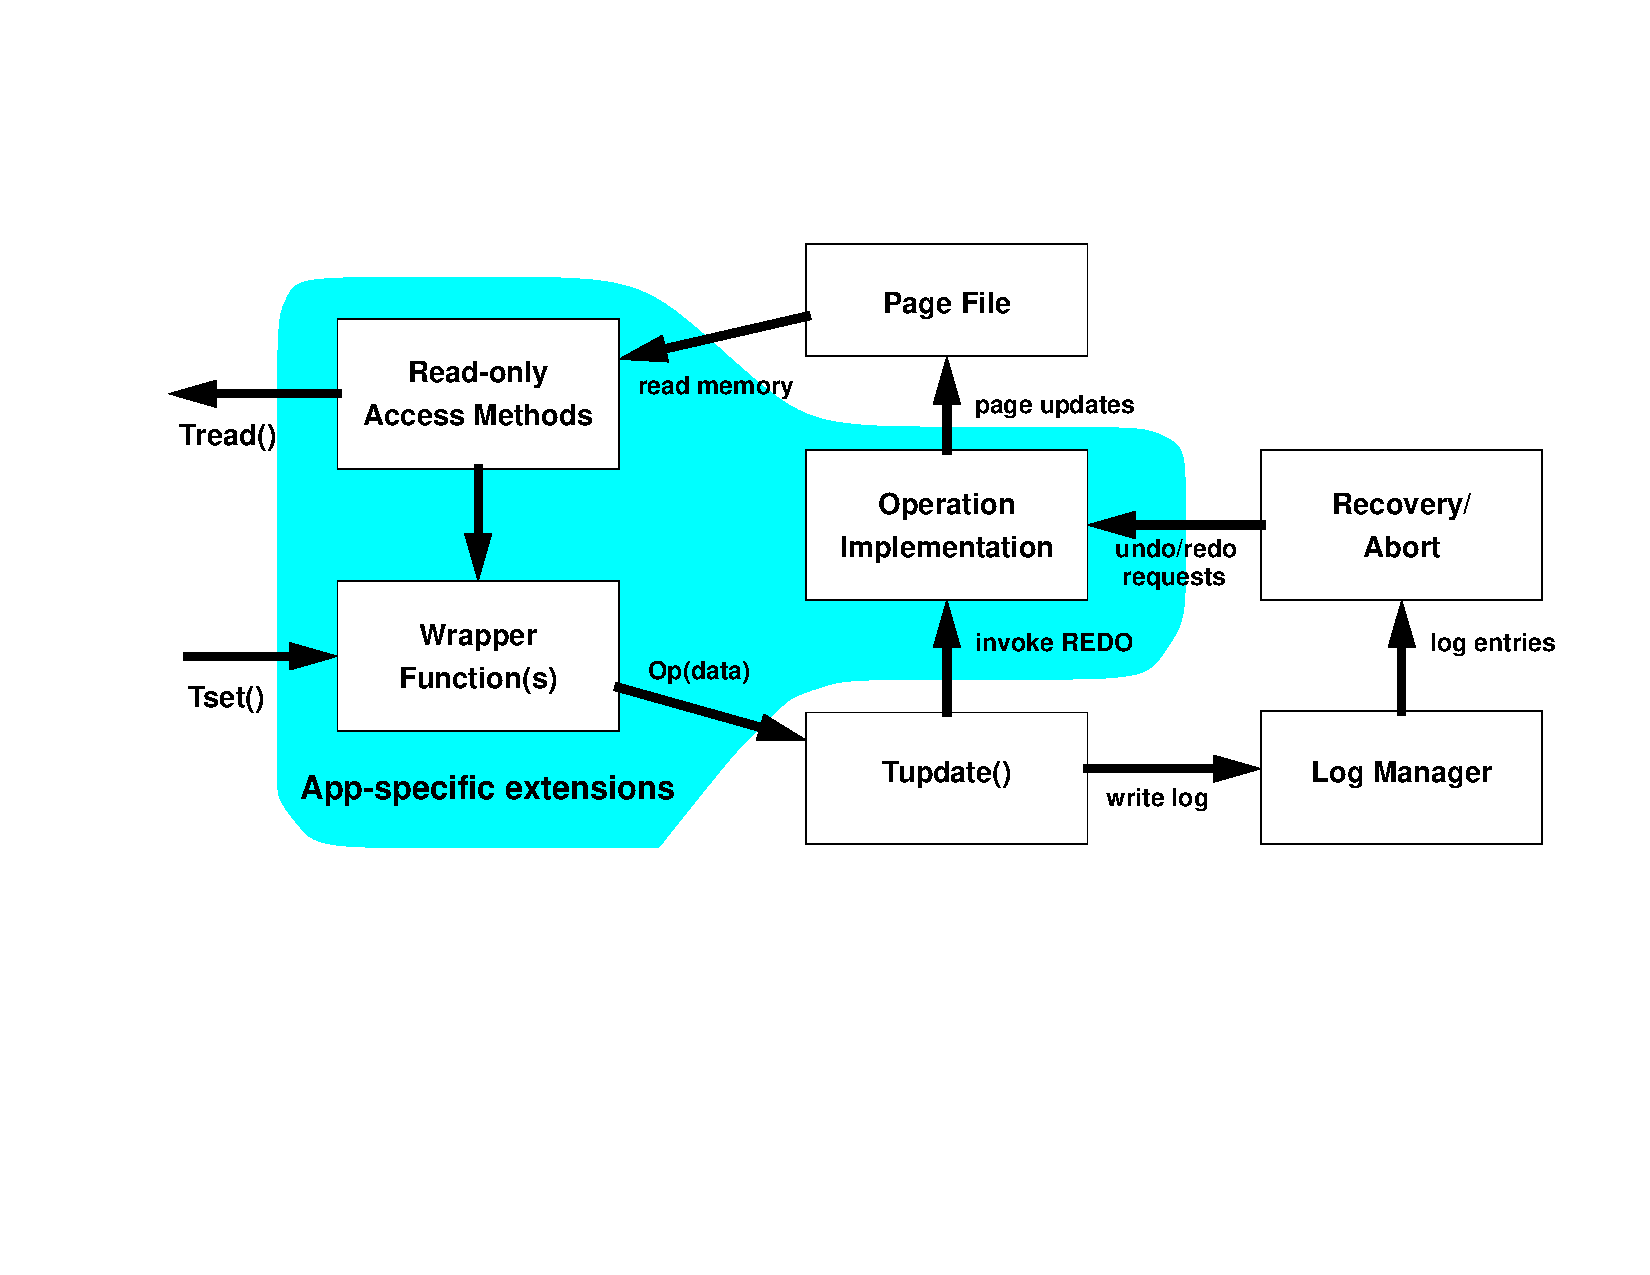
\includegraphics[%
   width=1\columnwidth]{structure.pdf}
\caption{\sf \label{fig:structure} Structure of an action...}
\end{figure}


As long as operation implementations obey the atomicity constraints
outlined above and the algorithms they use correctly manipulate
on-disk data structures, the write ahead logging protocol will provide
the application with the ACID transactional semantics, and provide
high performance, highly concurrent and scalable access to the
application data that is stored in the system.  This suggests a
natural partitioning of transactional storage mechanisms into two
parts.

The lower layer implements the write-ahead logging component,
including a buffer pool, logger, and (optionally) a lock manager.  
The complexity of the write-ahead logging component lies in
determining exactly when the UNDO and REDO operations should be
applied, when pages may be flushed to disk, log truncation, logging
optimizations, and a large number of other data-independent extensions
and optimizations.  This layer is the core of \yad.

The upper layer, which can be authored by the application developer,
provides the actual data structure implementations, policies regarding
page layout (other than the location of the LSN field), and the
implementation of any application-specific operations.  As long as
each layer provides well defined interfaces, the application,
operation implementation, and write-ahead logging component can be
independently extended and improved.

We have implemented a number of simple, high performance
and general-purpose data structures.  These are used by our sample
applications and as building blocks for new data structures.  Example
data structures include two distinct linked-list implementations, and
a growable array.  Surprisingly, even these simple operations have
important performance characteristics that are not available from
existing systems. 
%(Sections~\ref{sub:Linear-Hash-Table} and~\ref{TransClos})

The remainder of this section is devoted to a description of the
various primitives that \yad provides to application developers.

\subsection{Lock Manager}
\label{lock-manager}
%\eab{present the API?}

 \yad provides a default page-level lock manager that performs deadlock
detection, although we expect many applications to make use of
deadlock-avoidance schemes, which are already prevalent in
multithreaded application development.  The lock manager is flexible
enough to also provide index locks for hashtable implementations and 
more complex locking protocols such as hierarhical two-phase 
locking.~\cite{hierarcicalLocking,hierarchicalLockingOnAriesExample}  
The lock manager api is divided into callback functions that are made 
during normal operation and recovery, and into generic lock mananger 
implementations that may be used with \yad and its index implementations.

%For example, it would be relatively easy to build a strict two-phase
%locking hierarchical lock
%manager
% on
%top of \yad.  Such a lock manager would provide isolation guarantees
%for all applications that make use of it.  

However, applications that
make use of a lock manager must handle deadlocked transactions
that have been aborted by the lock manager.  This is easy if all of
the state is managed by \yad, but other state such as thread stacks
must be handled by the application, much like exception handling.  
\yad currently uses a custom wrapper around the pthread cancellation 
mechanism to provide partial stack unwinding and pthread's thread
cancellation mechanism.  Applications may use this error handling 
technique, or write simple wrappers to handle errors with the 
error handling scheme of their choice.

Conversely, many applications do not require such a general scheme.
If deadlock avoidance (``normal'' thread synchronization) can be used,
the application does not have to abort partial transactions, repeat
work, or deal with the corner cases that aborted transactions create.
%For instance, an IMAP server can employ a simple lock-per-folder
%approach and use lock-ordering techniques to avoid deadlock.  This
%avoids the complexity of dealing with transactions that abort due
%to deadlock, and also removes the runtime cost of restarting 
%transactions.

%\yad provides a lock manager API that allows all three variations
%(among others). In particular, it provides upcalls on commit/abort so
%that the lock manager can release locks at the right time. We will
%revisit this point in more detail when we describe some of the example
%operations.


%% @todo where does this text go??

%\subsection{Normal Processing}
%
%%% @todo draw the new version of this figure, with two boxes for the
%%% operation that interface w/ the logger and page file.
%
%Operation implementors follow the pattern in Figure \ref{cap:Tset},
%and need only implement a wrapper function (``Tset()'' in the figure,
%and register a pair of redo and undo functions with \yad.
%The Tupdate function, which is built into \yad, handles most of the
%runtime complexity.  \yad uses the undo and redo functions
%during recovery in the same way that they are used during normal
%processing.  
%
%The complexity of the ARIES algorithm lies in determining
%exactly when the undo and redo operations should be applied.  \yad 
%handles these details for the implementors of operations.
%
%
%\subsubsection{The buffer manager}
%
%\yad manages memory on behalf of the application and prevents pages
%from being stolen prematurely. Although \yad uses the STEAL policy
%and may write buffer pages to disk before transaction commit, it still
%must make sure that the UNDO log entries have been forced to disk
%before the page is written to disk. Therefore, operations must inform
%the buffer manager when they write to a page, and update the LSN of
%the page. This is handled automatically by the write methods that \yad 
%provides to operation implementors (such as writeRecord()). However,
%it is also possible to create your own low-level page manipulation
%routines, in which case these routines must follow the protocol.
%
%
%\subsubsection{Log entries and forward operation\\ (the Tupdate() function)\label{sub:Tupdate}}
%
%In order to handle crashes correctly, and in order to undo the
%effects of aborted transactions, \yad provides operation implementors
%with a mechanism to log undo and redo information for their actions.
%This takes the form of the log entry interface, which works as follows.
%Operations consist of a wrapper function that performs some pre-calculations
%and perhaps acquires latches. The wrapper function then passes a log
%entry to \yad. \yad passes this entry to the logger, {\em and then processes
%it as though it were redoing the action during recovery}, calling a function
%that the operation implementor registered with
%\yad. When the function returns, control is passed back to the wrapper
%function, which performs any post processing (such as generating return
%values), and releases any latches that it acquired. %
%\begin{figure}
%%\begin{center}
%%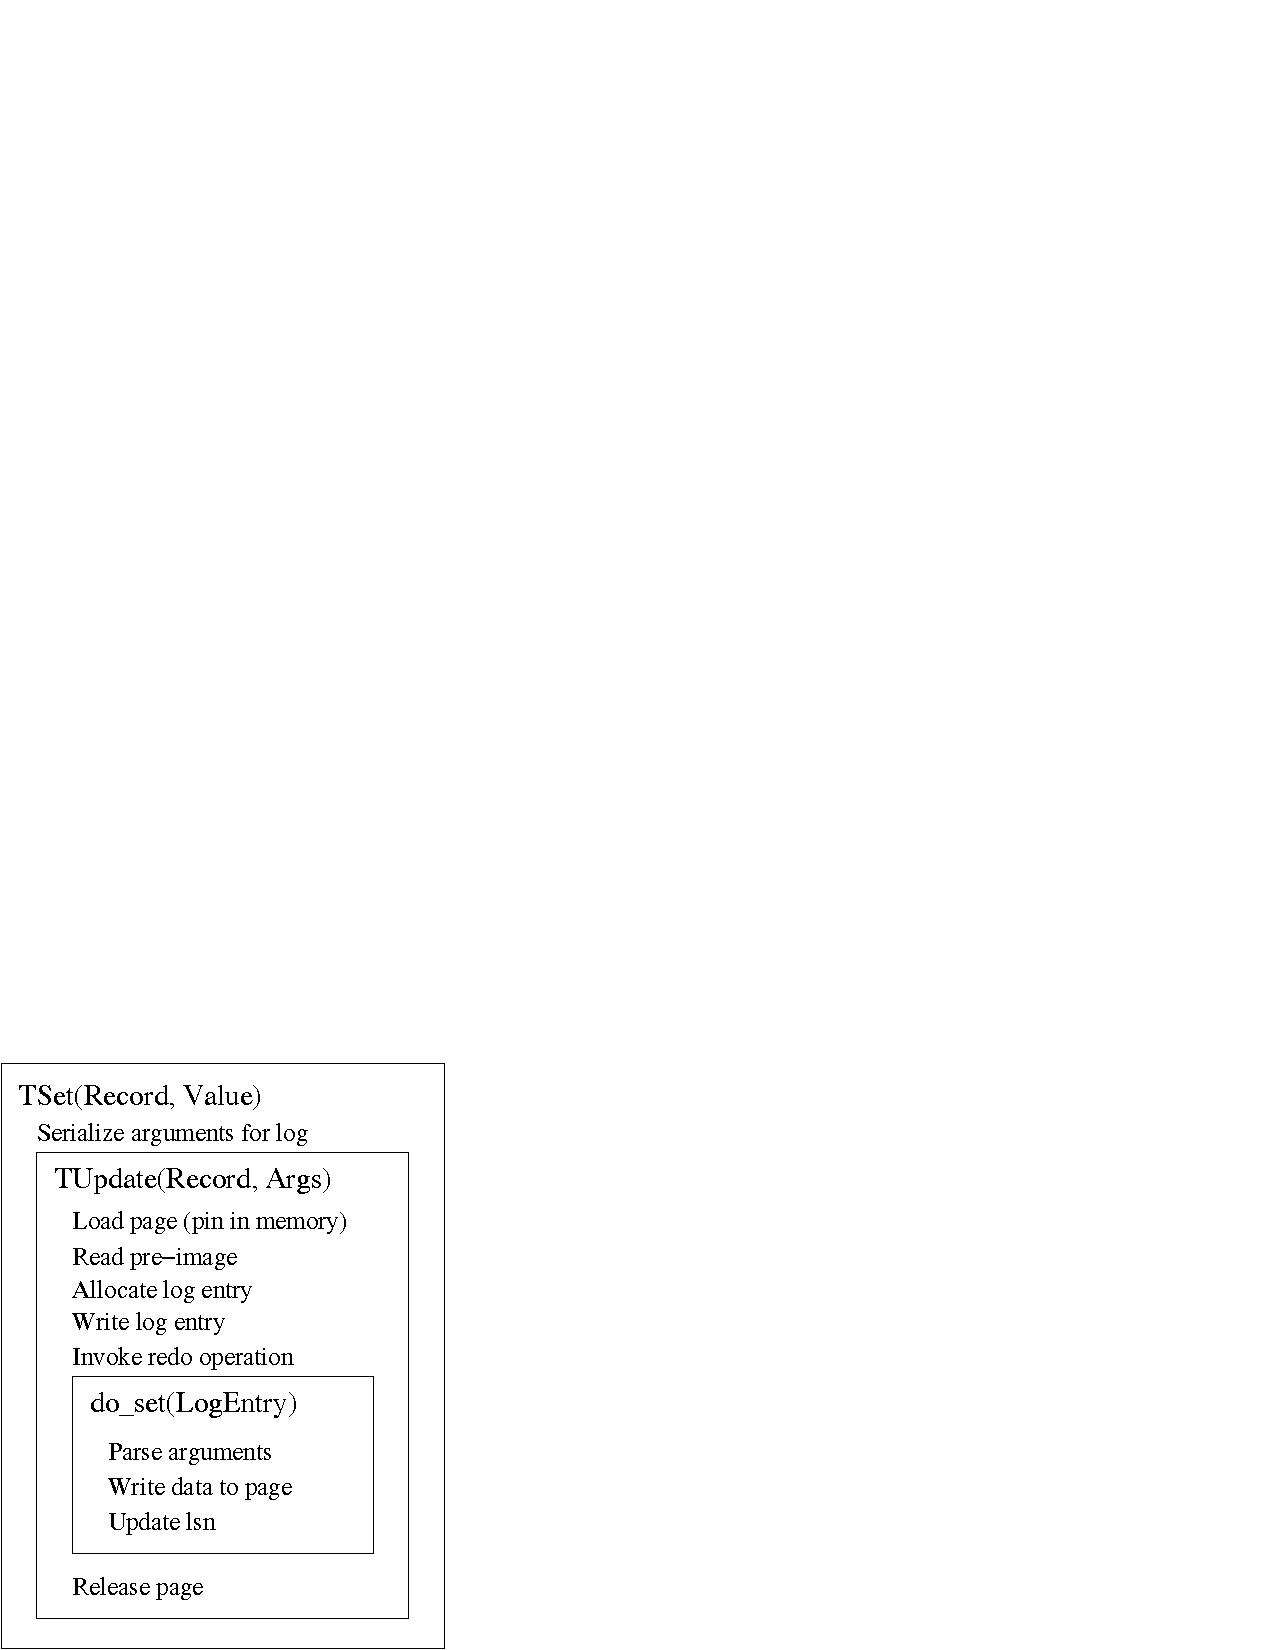
\includegraphics[%
%%  width=0.70\columnwidth]{TSetCall.pdf}
%%\end{center}
%
%\caption{\label{cap:Tset}Runtime behavior of a simple operation. Tset() and redoSet() are
%extensions that implement a new operation, while Tupdate() is built in. New operations
%need not be aware of the complexities of \yad.}
%\end{figure}
%
%This way, the operation's behavior during recovery's redo phase (an
%uncommon case) will be identical to the behavior during normal processing,
%making it easier to spot bugs. Similarly, undo and redo operations take
%an identical set of parameters, and undo during recovery is the same 
%as undo during normal processing.  This makes recovery bugs more obvious and allows redo
%functions to be reused to implement undo. 
%
%Although any latches acquired by the wrapper function will not be
%re acquired during recovery, the redo phase of the recovery process
%is single threaded. Since latches acquired by the wrapper function
%are held while the log entry and page are updated, the ordering of
%the log entries and page updates associated with a particular latch
%will be consistent. Because undo occurs during normal operation, 
%some care must be taken to ensure that undo operations obtain the 
%proper latches.
%

%\subsection{Summary}
%
%This section presented a relatively simple set of rules and patterns
%that a developer must follow in order to implement a durable, transactional
%and highly-concurrent data structure using \yad:

  % rcs:The last paper contained a tutorial on how to use \yad, which 
  % should be shortened or removed from this version, so I didn't paste it 
  % in.  However, it made some points that belong in this section
  % see: ##2##

%\begin{enumerate}
  %
  % need block diagram here.  4 blocks:
  %
  % App specific:
  %
  %  - operation wrapper
  %  - operation redo fcn
  %
  % \yad core:
  % 
  %  - logger
  %  - page file
  %
  % lock manager, etc can come later...
  %

%  \item {\bf {}``Write ahead logging protocol'' vs {}``Data structure implementation''}
%
%A \yad operation consists of some code that manipulates data that has
%been stored in transactional pages.  These operations implement
%high-level actions that are composed into transactions.  They are
%implemented at a relatively low level, and have full access to the
%ARIES algorithm.  Applications are implemented on top of the
%interfaces provided by an application-specific set of operations.
%This allows the the application, the operation, and \yad itself to be
%independently improved. 


\subsection{Flexible Logging and Page Layouts}
\label{flex-logging}
\label{page-layouts}

\yad supports three types of logging, and allows applications to create
{\em custom log entries} of each type.

%The overview discussion avoided the use of some common terminology 
%that should be presented here. 
{\em Physical logging } 
is the practice of logging physical (byte-level) updates
and the physical (page-number) addresses to which they are applied.

{\em Physiological logging } extends this idea, and is generally used 
for \yad's REDO entries.  The physical address (page number) is
stored, along with the arguments of an arbitrary function that 
is associated with the log entry.

This is used to implement many primatives, including {\em slotted pages}, which use
an on-page level of indirection to allow records to be rearranged
within the page; instead of using the page offset, REDO operations use
the index to locate the data within the page. This allows data within a single
page to be re-arranged easily, producing contiguous regions of
free space.  Since the log entry is associated with an arbitrary function
more sophisticated log entries can be implemented.  In turn, this can improve 
performance by conserving log space, or be used to build match recovery to application
semantics.
%\yad generalizes this model, allowing the parameters of a 
%custom log entry to invoke arbitrary application-specific code.  
%In 
%Section~\ref{OASYS} this is used to significantly improve performance by 
%storing difference records in an application specfic format.

%In addition to supporting custom log entries, this mechanism 
%is the basis of \yad's {\em flexible page layouts}.  
\yad also uses this mechanism to support four {\em page layouts}: 
{\em raw-page}, which is just an array of
bytes, {\em fixed-page}, a record-oriented page with fixed-length records,
{\em slotted-page}, which supports variable-sized records, and 
{\em versioned-page},  a slotted-page with a seperate version number for 
each record. (Section~\ref{version-pages}).  

{\em Logical logging} uses a higher-level key to specify the
UNDO/REDO.  Since these higher-level keys may affect multiple pages,
they are prohibited for REDO functions, since our REDO is specific to
a single page.  However, logical logging does make sense for UNDO,
since we can assume that the pages are physically consistent when we
apply an UNDO.  We thus use logical logging to undo operations that
span multiple pages, as shown in the next section.

%% can only be used for undo entries in \yad, and
%% stores a logical address (the key of a hash table, for instance)
%% instead of a physical address. As we will see later, these operations
%% may affect multiple pages.  This allows the location of data in the
%% page file to change, even if outstanding transactions may have to roll
%% back changes made to that data. Clearly, for \yad to be able to apply
%% logical log entries, the page file must be physically consistent,
%% ruling out use of logical logging for redo operations.

%\yad supports all three types of logging, and allows developers to
%register new operations, which we cover below.


\subsection{Nested Top Actions}
\label{nested-top-actions}

The operations presented so far work fine for a single page, since
each update is atomic.  For updates that span multiple pages there 
are two basic options: full isolation or nested top actions.

By full isolation, we mean that no other transactions see the
in-progress updates, which can be trivially achieved with a big lock
around the whole structure.  Usually the application must enforce 
such a locking policy or decide to use a lock manager and deal with 
deadlock.  Given isolation, \yad needs nothing else to
make multi-page updates transactional: although many pages might be
modified they will commit or abort as a group and be recovered
accordingly.

However, this level of isolation disallows all concurrency between 
transactions that use the same data structure.  ARIES introduced the 
notion of nested top actions to
address this problem.  For example, consider what would happen if one
transaction, $A$, rearranged the layout of a data structure, a second
transaction, $B$, added a value to the rearranged structure, and then
the first transaction aborted.  (Note that the structure is not
isolated.)  While applying physical undo information to the altered
data structure,  $A$ would UNDO its writes
without considering the modifications made by
$B$, which is likely to cause corruption.  Therefore, $B$ would 
have to be aborted as well ({\em cascading aborts}).

With nested top actions, ARIES defines the structural changes as a
mini-transaction. This means that the structural change
``commits'' even if the containing transaction ($A$) aborts, which
ensures that $B$'s update remains valid.

\yad supports nested atomic actions as the preferred way to build
high-performance data structures. In particular, an operation that
spans pages can be made atomic by simply wrapping it in a nested top
action and obtaining appropriate latches at runtime.  This approach
reduces development of atomic page spanning operations to something
very similar to conventional multithreaded development that use mutexes
for synchronization.
In particular, we have found a simple recipe for converting a
non-concurrent data structure into a concurrent one, which involves
three steps:
\begin{enumerate}
\item Wrap a mutex around each operation.  If this is done with care,
  it may be possible to use finer grained mutexes.
\item Define a logical UNDO for each operation (rather than just using
  a lower-level physical UNDO).  For example, this is easy for a
  hashtable; e.g. the UNDO for an {\em insert} is {\em remove}.
\item For mutating operations (not read-only), add a ``begin nested
  top action'' right after the mutex acquisition, and a ``commit
  nested top action'' right before the mutex is released.
\end{enumerate}
This recipe ensures that operations that might span multiple pages
atomically apply and commit any structural changes and thus avoids 
cascading aborts.  If the transaction that encloses the operations
aborts, the logical undo will {\em compensate} for
its effects, but leave its structural changes intact. Because this 
recipe does not ensure transactional consistency and is largely 
orthoganol to the use of a lock mananger, we call this class of 
concurrenct control {\em latching} throughout this paper.

We have found the recipe to be easy to follow and very effective, and
we use it everywhere our concurrent data structures may make structural 
changes, such as growing a hash table or array.

%% \textcolor{red}{OLD TEXT:} Section~\ref{sub:OperationProperties} states that \yad does not allow
%% cascading aborts, implying that operation implementors must protect
%% transactions from any structural changes made to data structures by
%% uncommitted transactions, but \yad does not provide any mechanisms
%% designed for long-term locking. However, one of \yad's goals is to
%% make it easy to implement custom data structures for use within safe,
%% multi-threaded transactions. Clearly, an additional mechanism is
%% needed.

%% The solution is to allow portions of an operation to ``commit'' before
%% the operation returns.\footnote{We considered the use of nested top actions, which \yad could easily
%% support. However, we currently use the slightly simpler (and lighter-weight)
%% mechanism described here. If the need arises, we will add support
%% for nested top actions.}
%% An operation's wrapper is just a normal function, and therefore may
%% generate multiple log entries. First, it writes an UNDO-only entry
%% to the log. This entry will cause the \emph{logical} inverse of the
%% current operation to be performed at recovery or abort, must be idempotent,
%% and must fail gracefully if applied to a version of the database that
%% does not contain the results of the current operation. Also, it must
%% behave correctly even if an arbitrary number of intervening operations
%% are performed on the data structure.

%% Next, the operation writes one or more redo-only log entries that may
%% perform structural modifications to the data structure. These redo
%% entries have the constraint that any prefix of them must leave the
%% database in a consistent state, since only a prefix might execute
%% before a crash.  This is not as hard as it sounds, and in fact the
%% $B^{LINK}$ tree~\cite{blink} is an example of a B-Tree implementation
%% that behaves in this way, while the linear hash table implementation
%% discussed in Section~\ref{sub:Linear-Hash-Table} is a scalable hash
%% table that meets these constraints.

%% %[EAB: I still think there must be a way to log all of the redoes
%% %before any of the actions take place, thus ensuring that you can redo
%% %the whole thing if needed. Alternatively, we could pin a page until
%% %the set completes, in which case we know that that all of the records
%% %are in the log before any page is stolen.]



\subsection{Adding Log Operations}
\label{op-def}

%  \item {\bf  ARIES provides {}``transactional pages'' }

Given this background, we now cover adding new operations. \yad is
designed to allow application developers to easily add new data
representations and data structures by defining new operations.

There are a number of invariants that these operations must obey:
\begin{enumerate}
\item Pages should only be updated inside of a REDO or UNDO function.
\item An update to a page atomically updates the LSN by pinning the page.
\item If the data read by the wrapper function must match the state of
the page that the REDO function sees, then the wrapper should latch
the relevant data.
\item REDO operations use page numbers and possibly record numbers
while UNDO operations use these or logical names/keys
\item Acquire latches as needed (typically per page or record)
\item Use nested top actions (which require a logical UNDO log record) 
or ``big locks'' (which drastically reduce concurrency) for multi-page updates.
\end{enumerate}

\noindent{\bf An Example: Increment/Decrement}

A common optimization for TPC benchmarks is to provide hand-built
operations that support adding/subtracting from an account.  Such
operations improve concurrency since they can be reordered and can be
easily made into nested top actions (since the logical UNDO is
trivial). Here we show how increment/decrement map onto \yad operations.

First, we define the operation-specific part of the log record:
\begin{small}
\begin{verbatim}
typedef struct { int amount } inc_dec_t;
\end{verbatim}
\noindent {\normalsize Here is the increment operation; decrement is
analogous:}
\begin{verbatim}
// p is the bufferPool's current copy of the page.
int operateIncrement(int xid, Page* p, lsn_t lsn,
                     recordid rid, const void *d) {
  inc_dec_t * arg = (inc_dec_t)d;
  int i;
  latchRecord(rid); 
  readRecord(xid, p, rid, &i);   // read current value
  i += arg->amount;
  
  // write new value and update the LSN
  writeRecord(xid, p, lsn, rid, &i);
  unlatchRecord(rid); 
  return 0;                      // no error
}
\end{verbatim}
\noindent{\normalsize Next, we register the operation:}
\begin{verbatim}
// first set up the normal case
ops[OP_INCREMENT].implementation= &operateIncrement;
ops[OP_INCREMENT].argumentSize  = sizeof(inc_dec_t);

// set the REDO to be the same as normal operation
//   Sometime is useful to have them differ.
ops[OP_INCREMENT].redoOperation = OP_INCREMENT;

// set UNDO to be the inverse
ops[OP_INCREMENT].undoOperation = OP_DECREMENT;
\end{verbatim}
{\normalsize Finally, here is the wrapper that uses the
operation, which is identified via {\small\tt OP\_INCREMENT};
applications use the wrapper rather than the operation, as it tends to
be cleaner.}
\begin{verbatim}
int Tincrement(int xid, recordid rid, int amount) {
   // rec will be serialized to the log.
   inc_dec_t rec;
   rec.amount = amount;

   // write a log entry, then execute it
   Tupdate(xid, rid, &rec, OP_INCREMENT);

   // return the incremented value
   int new_value;
   // wrappers can call other wrappers
   Tread(xid, rid, &new_value);
   return new_value;
}
\end{verbatim}
\end{small}


With some examination it is possible to show that this example meets
the invariants.  In addition, because the REDO code is used for normal
operation, most bugs are easy to find with conventional testing
strategies.  
% covered this in future work...
%As future work, there is some hope of verifying these
%invariants statically; for example, it is easy to verify that pages
%are only modified by operations, and it is also possible to verify
%latching for our page layouts that support records.

%% Furthermore, we plan to develop a number of tools that will
%% automatically verify or test new operation implementations' behavior
%% with respect to these constraints, and behavior during recovery.  For
%% example, whether or not nested top actions are used, randomized
%% testing or more advanced sampling techniques~\cite{OSDIFSModelChecker}
%% could be used to check operation behavior under various recovery
%% conditions and thread schedules.

However, as we will see in Section~\ref{OASYS}, even these invariants
can be stretched by sophisticated developers.

\subsection{Summary}

In this section we walked through some of the more important parts of
the \yad API, including the lock manager, nested top actions and log
operations.  The majority of the recovery algorithm's complexity is 
hidden from developers.  We argue that \yad's novel approach toward 
the encapsulation of transactional primatives makes it easy for 
developers to use these mechanisms to enhance application performance
and simplify software design.

%\eab{update}
%The ARIES algorithm is extremely complex, and we have left
%out most of the details needed to understand how ARIES works. Yet, we 
%have covered the information that is needed to implement new
%transactional data structures.  \yad's encapsulation of ARIES makes 
%this possible, and was performed in a way that strongly differentiates
%\yad from existing systems.


%We hope that this will increase the availability of transactional
%data primitives to application developers.



%\begin{enumerate}

%  \item {\bf Log entries as a programming primitive }

  %rcs: Not quite happy with existing text; leaving this section out for now.
  %
  %  Need to make some points the old text did not make:
  %
  %     - log optimizations (for space) can be very important.  
  %           - many small writes 
  %           - large write of small diff 
  %           - app overwrites page many times per transaction (for example, database primary key)
  %    We have solutions to #1 and 2.  A general solution to #3 involves 'scrubbing' a logical log of redundant operations.
  %    
  %        - Talk about virtual async log thing...
  %           - reordering
  %           - distribution

%  \item {\bf Error handling with compensations as {}``abort() for C''}

  % stylized usage of Weimer -> cheap error handling, no C compiler modifications...

%  \item {\bf Concurrency models are fundamentally application specific, but
%  record/page level locking and index locks are often a nice trade-off}  @todo We sort of cover this above

%  \item {\bf {}``latching'' vs {}``locking'' - data structures internal to
%  \yad are protected by \yad, allowing applications to reason in
%  terms of logical data addresses, not physical representation. Since
%  the application may define a custom representation, this seems to be
%  a reasonable tradeoff between application complexity and
%  performance.}
%
%  \item {\bf Non-interleaved transactions vs. Nested top actions
%  vs. Well-ordered writes.}

    % key point: locking + nested top action = 'normal' multithreaded
    %software development! (modulo 'obvious' mistakes like algorithmic
    %errors in data structures, errors in the log format, etc)
    
    % second point: more difficult techniques can be used to optimize
    % log bandwidth. _in ways that other techniques cannot provide_ 
    % to application developers.



%\end{enumerate}

%\section{Other operations (move to the end of the paper?)}
%
%\begin{enumerate}
%
%  \item {\bf Atomic file-based transactions. 
%    
%    Prototype blob implementation  using force, shadow copies (it is trivial to implement given transactional
%  pages).  
%
%  File systems that implement atomic operations may allow
%  data to be stored durably without calling flush() on the data
%  file. 
%
%  Current implementation useful for blobs that are typically
%  changed entirely from update to update, but smarter implementations
%  are certainly possible. 
%
%  The blob implementation primarily consists
%  of special log operations that cause file system calls to be made at
%  appropriate times, and is simple, so it could easily be replaced by
%  an application that frequently update small ranges within blobs, for
%  example.}

%\subsection{Array List}
   % Example of how to avoid nested top actions
%\subsection{Linked Lists}
   % Example of two different page allocation strategies.
   % Explain how to implement linked lists w/out NTA's (even though we didn't do that)?

%\subsection{Linear Hash Table\label{sub:Linear-Hash-Table}}
%   % The implementation has changed too much to directly reuse old section, other than description of linear hash tables:
%
%Linear hash tables are hash tables that are able to extend their bucket
%list incrementally at runtime. They work as follows. Imagine that
%we want to double the size of a hash table of size $2^{n}$, and that
%the hash table has been constructed with some hash function $h_{n}(x)=h(x)\, mod\,2^{n}$.
%Choose $h_{n+1}(x)=h(x)\, mod\,2^{n+1}$ as the hash function for
%the new table. Conceptually we are simply prepending a random bit
%to the old value of the hash function, so all lower order bits remain
%the same. At this point, we could simply block all concurrent access
%and iterate over the entire hash table, reinserting values according
%to the new hash function. 
%
%However, because of the way we chose $h_{n+1}(x),$ we know that the
%contents of each bucket, $m$, will be split between bucket $m$ and
%bucket $m+2^{n}$. Therefore, if we keep track of the last bucket that
%was split, we can split a few buckets at a time, resizing the hash
%table without introducing long pauses while we reorganize the hash
%table~\cite{lht}. 
%
%We can handle overflow using standard techniques;
%\yad's linear hash table simply uses the linked list implementations
%described above.  The bucket list is implemented by reusing the array
%list implementation described above.
%
%% Implementation simple!  Just slap together the stuff from the prior two sections, and add a header + bucket locking.
%
%  \item {\bf Asynchronous log implementation/Fast
%  writes. Prioritization of log writes (one {}``log'' per page)
%  implies worst case performance (write, then immediate read) will
%  behave on par with normal implementation, but writes to portions of
%  the database that are not actively read should only increase system
%  load (and not directly increase latency)} This probably won't go
%  into the paper.  As long as the buffer pool isn't thrashing, this is
%  not much better than upping the log buffer.
%
%  \item {\bf Custom locking. Hash table can support all of the SQL
%  degrees of transactional consistency, but can also make use of
%  application-specific invariants and synchronization to accommodate
%  deadlock-avoidance, which is the model most naturally supported by C
%  and other programming languages.}  This is covered above, but we
%  might want to mention that we have a generic lock manager
%  implementation that operation implementors can reuse.  The argument
%  would be stronger if it were a generic hierarchical lock manager.

%Many plausible lock managers, can do any one you want.
%too much implemented part of DB; need more 'flexible' substrate.

%\end{enumerate}

\section{Experimental setup}
\label{sec:experimental_setup}

The following sections describe the design and implementation of
non-trivial functionality using \yad, and use Berkeley DB for
comparison where appropriate.  We chose Berkeley DB because, among
commonly used systems, it provides transactional storage that is most
similar to \yad, and it was
designed for high-performance, high-concurrency environments.

All benchmarks were run on an Intel Xeon 2.8 GHz with 1GB of RAM and a
10K RPM SCSI drive, formatted with reiserfs\footnote{We found that the
relative performance of Berkeley DB and \yad is highly sensitive to
filesystem choice, and we plan to investigate the reasons why the
performance of \yad under ext3 is degraded. However, the results
relating to the \yad optimizations are consistent across filesystem
types.}.  All reported numbers correspond to the mean of multiple runs
with a 95\% confidence interval with a half-width of 5\%.

We used Berkeley DB 4.2.52 as it existed in Debian Linux's testing
branch during March of 2005, with the flags DB\_TXN\_SYNC, and DB\_THREAD
enabled. These flags were chosen to match 
Berkeley DB's configuration to \yad's as closely as possible.  In cases where
Berkeley DB implements a feature that is not provided by \yad, we
enable the feature if it improves Berkeley DB's performance, but
disable the feature if it degrades Berkeley DB's performance.
For each of the tests, the two libraries provide the same transactional semantics.
%  With 
%the exception of \yad's optimized serialization mechanism in the 
%\oasys test (see Section \ref{OASYS}), 
%the two libraries provide the same set of transactional 
%semantics during each test.  

Optimizations to Berkeley DB that we performed included disabling the
lock manager, though we still use ``Free Threaded'' handles for all
tests.  This yielded a significant increase in performance because it
removed the possibility of transaction deadlock, abort, and repetition.
However, after introducing this optimization, highly concurrent
Berkeley DB benchmarks became unstable, suggesting either a bug or
misuse of the feature.  We believe that this problem would only
improve Berkeley DB's performance in our benchmarks, so we disabled
the lock manager for all tests.  Without this optimization, Berkeley
DB's performance for Figure~\ref{fig:TPS} strictly decreases with increased concurrency due to contention and deadlock recovery.

We increased Berkeley DB's buffer cache and log buffer sizes to match
\yad's default sizes.  Running with \yad's (larger) default values
roughly doubled Berkeley DB's performance on the bulk loading tests.

Finally, we would like to point out that we expended a considerable
effort tuning Berkeley DB, and that our efforts significantly
improved Berkeley DB's performance on these tests.  Although further
tuning by Berkeley DB experts might improve Berkeley DB's
numbers, we think that we have produced a reasonably fair comparison
between the two systems.  The source code and scripts we used to
generate this data is publicly available, and we have been able to
reproduce the trends reported here on multiple systems.


\section{Linear Hash Table\label{sub:Linear-Hash-Table}}


%\subsection{Conventional workloads}

%Existing database servers and transactional libraries are tuned to
%support OLTP (Online Transaction Processing) workloads well.  Roughly
%speaking, the workload of these systems is dominated by short
%transactions and response time is important.  
%
%We are confident that a
%sophisticated system based upon our approach to transactional storage
%will compete well in this area, as our algorithm is based upon ARIES,
%which is the foundation of IBM's DB/2 database.  However, our current
%implementation is geared toward simpler, specialized applications, so
%we cannot verify this directly.  Instead, we present a number of
%microbenchmarks that compare our system against Berkeley DB, the most
%popular transactional library.  Berkeley DB is a mature product and is
%actively maintained.  While it currently provides more functionality
%than our current implementation, we believe that our architecture
%could support a broader range of features than those that are provided 
%by BerkeleyDB's monolithic interface.

Hash table indices are common in databases and are also applicable to
a large number of applications.  In this section, we describe how we
implemented two variants of linear hash tables on top of \yad and
describe how \yad's flexible page and log formats enable interesting
optimizations.  We also argue that \yad makes it trivial to produce
concurrent data structure implementations.
%, and provide a set of
%mechanical steps that will allow a non-concurrent data structure
%implementation to be used by interleaved transactions.

Finally, we describe a number of more complex optimizations and
compare the performance of our optimized implementation, the
straightforward implementation and Berkeley DB's hash implementation.
The straightforward implementation is used by the other applications
presented in this paper and is \yad's default hashtable
implementation.  We chose this implementation over the faster optimized
hash table in order to this emphasize that it is easy to implement
high-performance transactional data structures with \yad and because
it is easy to understand.

We decided to implement a {\em linear} hash table~\cite{lht}.  Linear
hash tables are hash tables that are able to extend their bucket list
incrementally at runtime. They work as follows. Imagine that we want
to double the size of a hash table of size $2^{n}$ and that the hash
table has been constructed with some hash function $h_{n}(x)=h(x)\,
mod\,2^{n}$.  Choose $h_{n+1}(x)=h(x)\, mod\,2^{n+1}$ as the hash
function for the new table. Conceptually, we are simply prepending a
random bit to the old value of the hash function, so all lower order
bits remain the same. At this point, we could simply block all
concurrent access and iterate over the entire hash table, reinserting
values according to the new hash function.

However, 
%because of the way we chose $h_{n+1}(x),$ 
we know that the contents of each bucket, $m$, will be split between
bucket $m$ and bucket $m+2^{n}$. Therefore, if we keep track of the
last bucket that was split then we can split a few buckets at a time,
resizing the hash table without introducing long pauses~\cite{lht}.

In order to implement this scheme we need two building blocks.  We
need a map from bucket number to bucket contents (lists), and we need to handle bucket overflow.


\subsection{The Bucket Map}

The simplest bucket map would simply use a fixed-length transactional
array. However, since we want the size of the table to grow, we should
not assume that it fits in a contiguous range of pages. Instead, we build
on top of \yad's transactional ArrayList data structure (inspired by
Java's structure of the same name).

The ArrayList provides the appearance of large growable array by
breaking the array into a tuple of contiguous page intervals that
partition the array.  Since we expect relatively few partitions (one
per enlargement typically), this leads to an efficient map. We use a
single ``header'' page to store the list of intervals and their sizes.

For space efficiency, the array elements themselves are stored using
the fixed-length record page layout. Thus, we use the header page to
find the right interval, and then index into it to get the $(page,
slot)$ address.  Once we have this address, the REDO/UNDO entries are
trivial: they simply log the before and after image of the that
record.


%\rcs{This paragraph doesn't really belong}
%Normal \yad slotted pages are not without overhead.  Each record has
%an associated size field, and an offset pointer that points to a
%location within the page.  Throughout our bucket list implementation,
%we only deal with fixed-length slots.  Since \yad supports multiple
%page layouts, we use the ``Fixed Page'' layout, which implements a
%page consisting on an array of fixed-length records.  Each bucket thus
%maps directly to one record, and it is trivial to map bucket numbers
%to record numbers within a page.  

%\yad provides a call that allocates a contiguous range of pages.  We
%use this method to allocate increasingly larger regions of pages as
%the array list expands, and store the regions' offsets in a single 
%page header.  

%When we need to access a record, we first calculate 
%which region the record is in, and use the header page to determine 
%its offset.  We can do this because the size of each region is 
%deterministic; it is simply $size_{first~region} * 2^{region~number}$.  
%We then calculate the $(page,slot)$ offset within that region.  


\subsection{Bucket List}

%\eab{don't get this section, and it sounds really complicated, which is counterproductive at this point  -- Is this better now? -- Rusty}
%
%\eab{some basic questions: 1) does the record described above contain
%key/value pairs or a pointer to a linked list?  Ideally it would be
%one bucket with a next pointer at the end... 2) what about values that
%are bigger than one bucket?, 3) add caption to figure.}

\begin{figure}
\hspace{.25in}
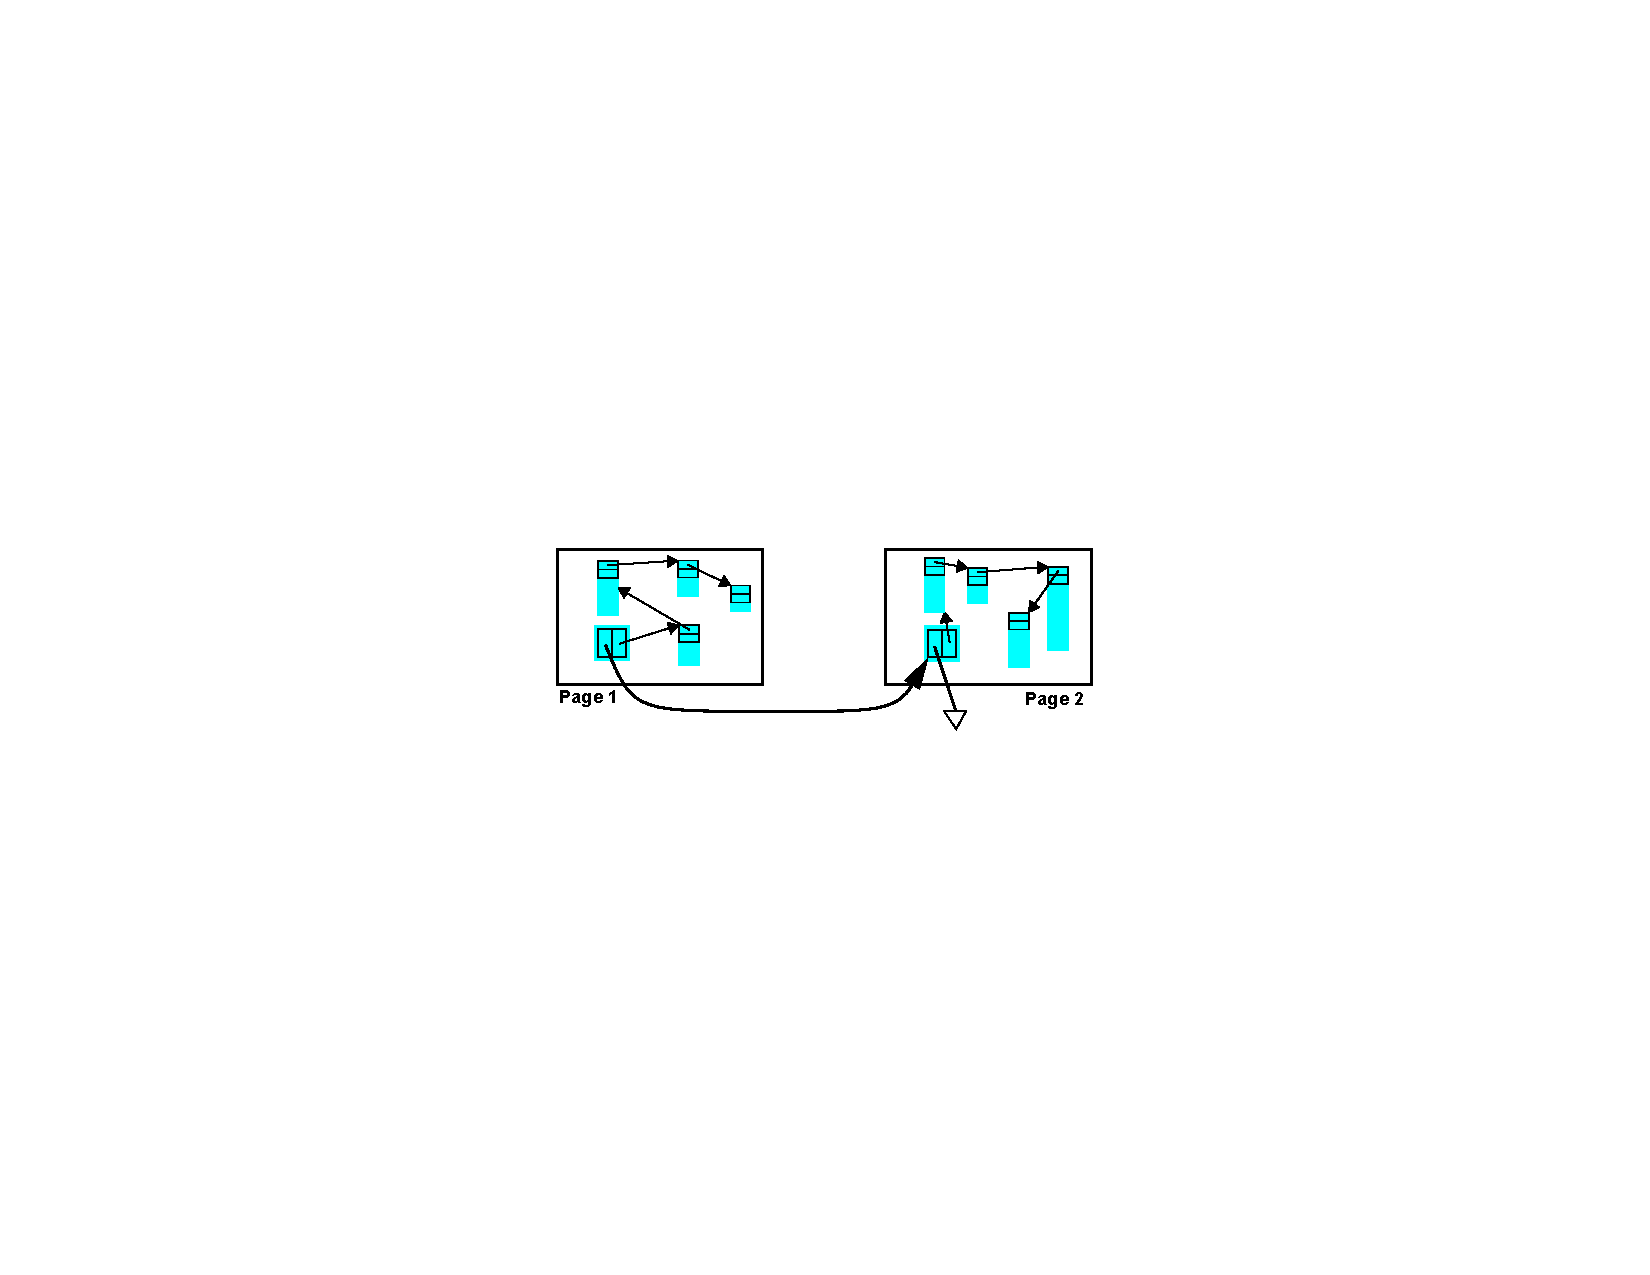
\includegraphics[width=3.25in]{LHT2.pdf}
\caption{\sf \label{fig:LHT}Structure of locality preserving ({\em page-oriented}) 
linked lists.  Hashtable bucket overflow lists tend to be of some small fixed 
length.  This data structure allows \yad to aggressively maintain page locality 
for short lists, providing fast overflow bucket traversal for the hash table.}
\end{figure}

Given the map, which locates the bucket, we need a transactional
linked list for the contents of the bucket.  The trivial implementation
would just link variable-size records together, where each record
contains a $(key,value)$ pair and the $next$ pointer, which is just a
$(page,slot)$ address.

However, in order to achieve good locality, we instead implement a
{\em page-oriented} transactional linked list, shown in
Figure~\ref{fig:LHT}.  The basic idea is to place adjacent elements of
the list on the same page: thus we use a list of lists. The main list
links pages together, while the smaller lists reside with that
page. \yad's slotted pages allows the smaller lists to support
variable-size values, and allow list reordering and value resizing
with a single log entry (since everything is on one page).

In addition, all of the entries within a page may be traversed without
unpinning and repinning the page in memory, providing very fast
traversal over lists that have good locality.  This optimization would
not be possible if it were not for the low-level interfaces provided
by the buffer manager.  In particular, we need to specify which page 
we would like to allocate space from and we need to be able to
read and write multiple records with a single call to pin/unpin.  Due to
this data structure's nice locality properties and good performance
for short lists, it can also be used on its own.

\begin{figure*}
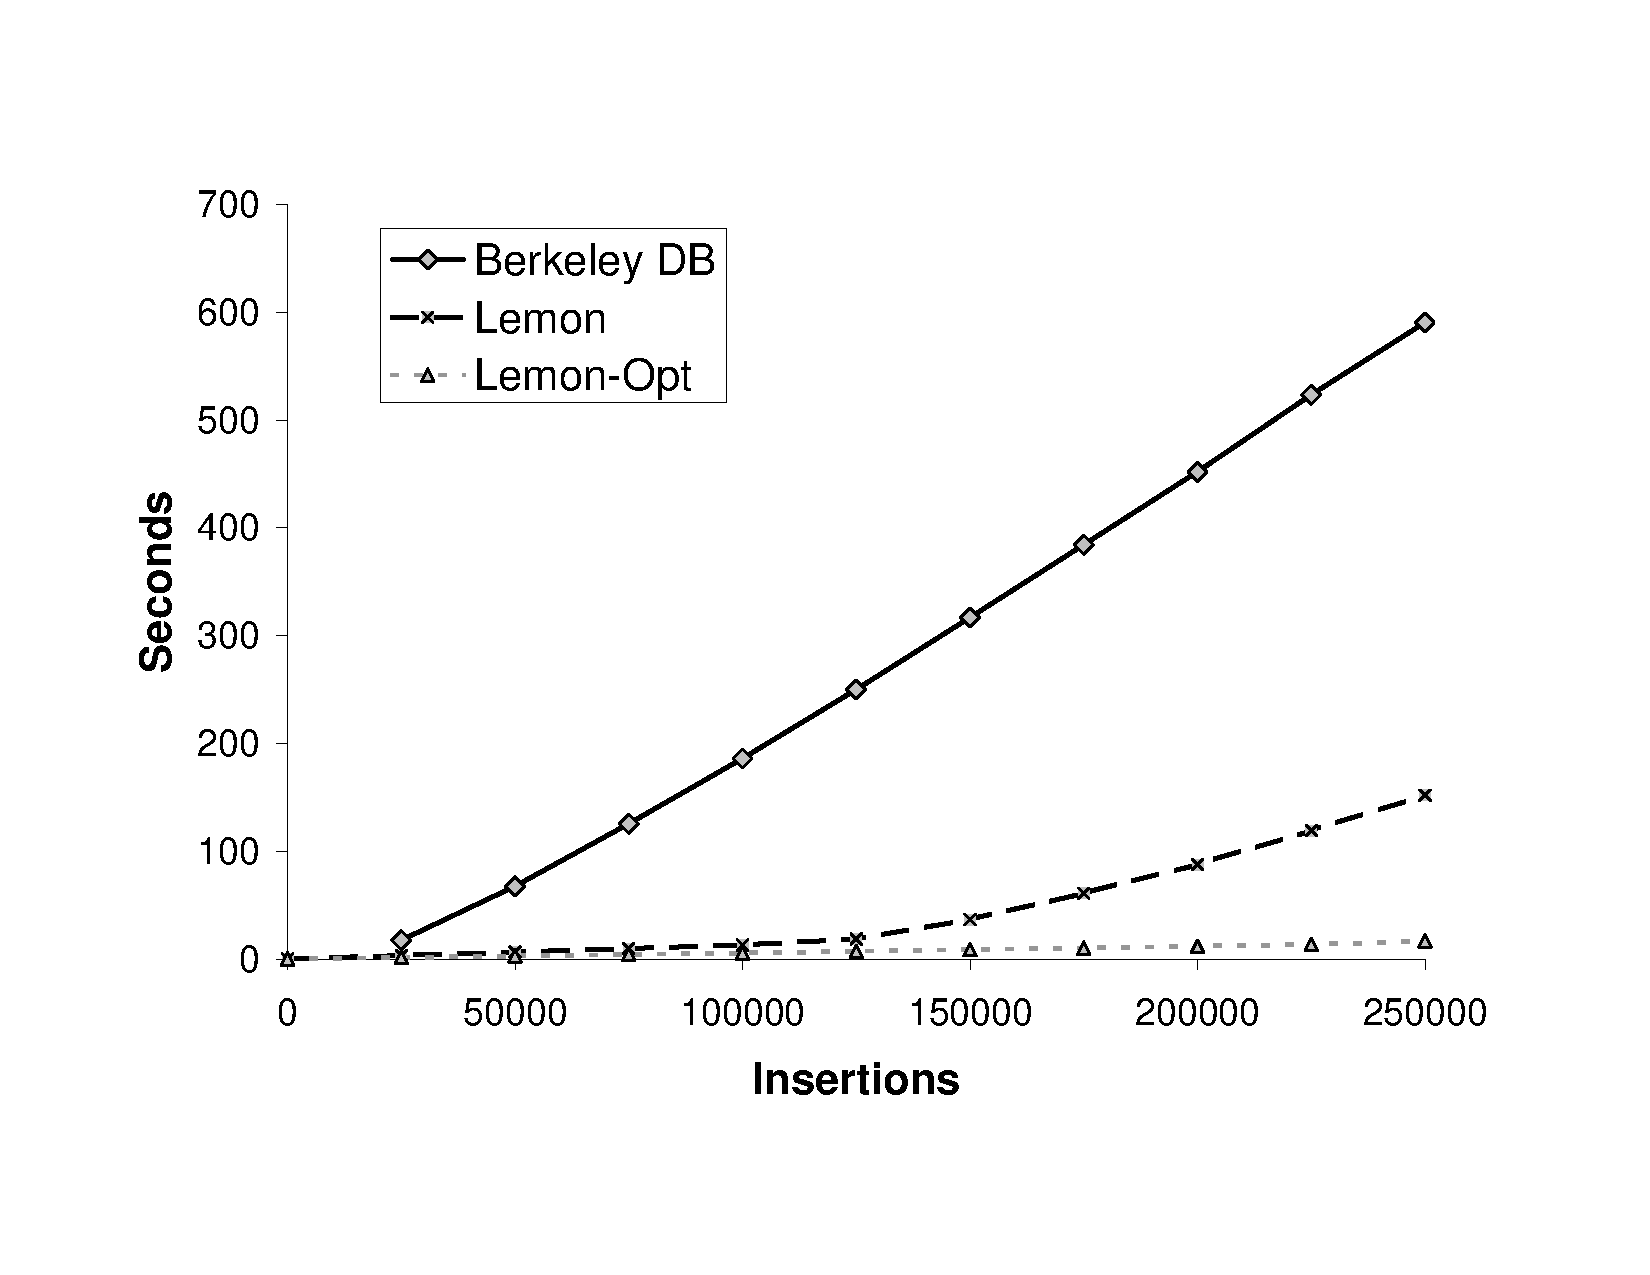
\includegraphics[%
   width=1\columnwidth]{bulk-load.pdf}
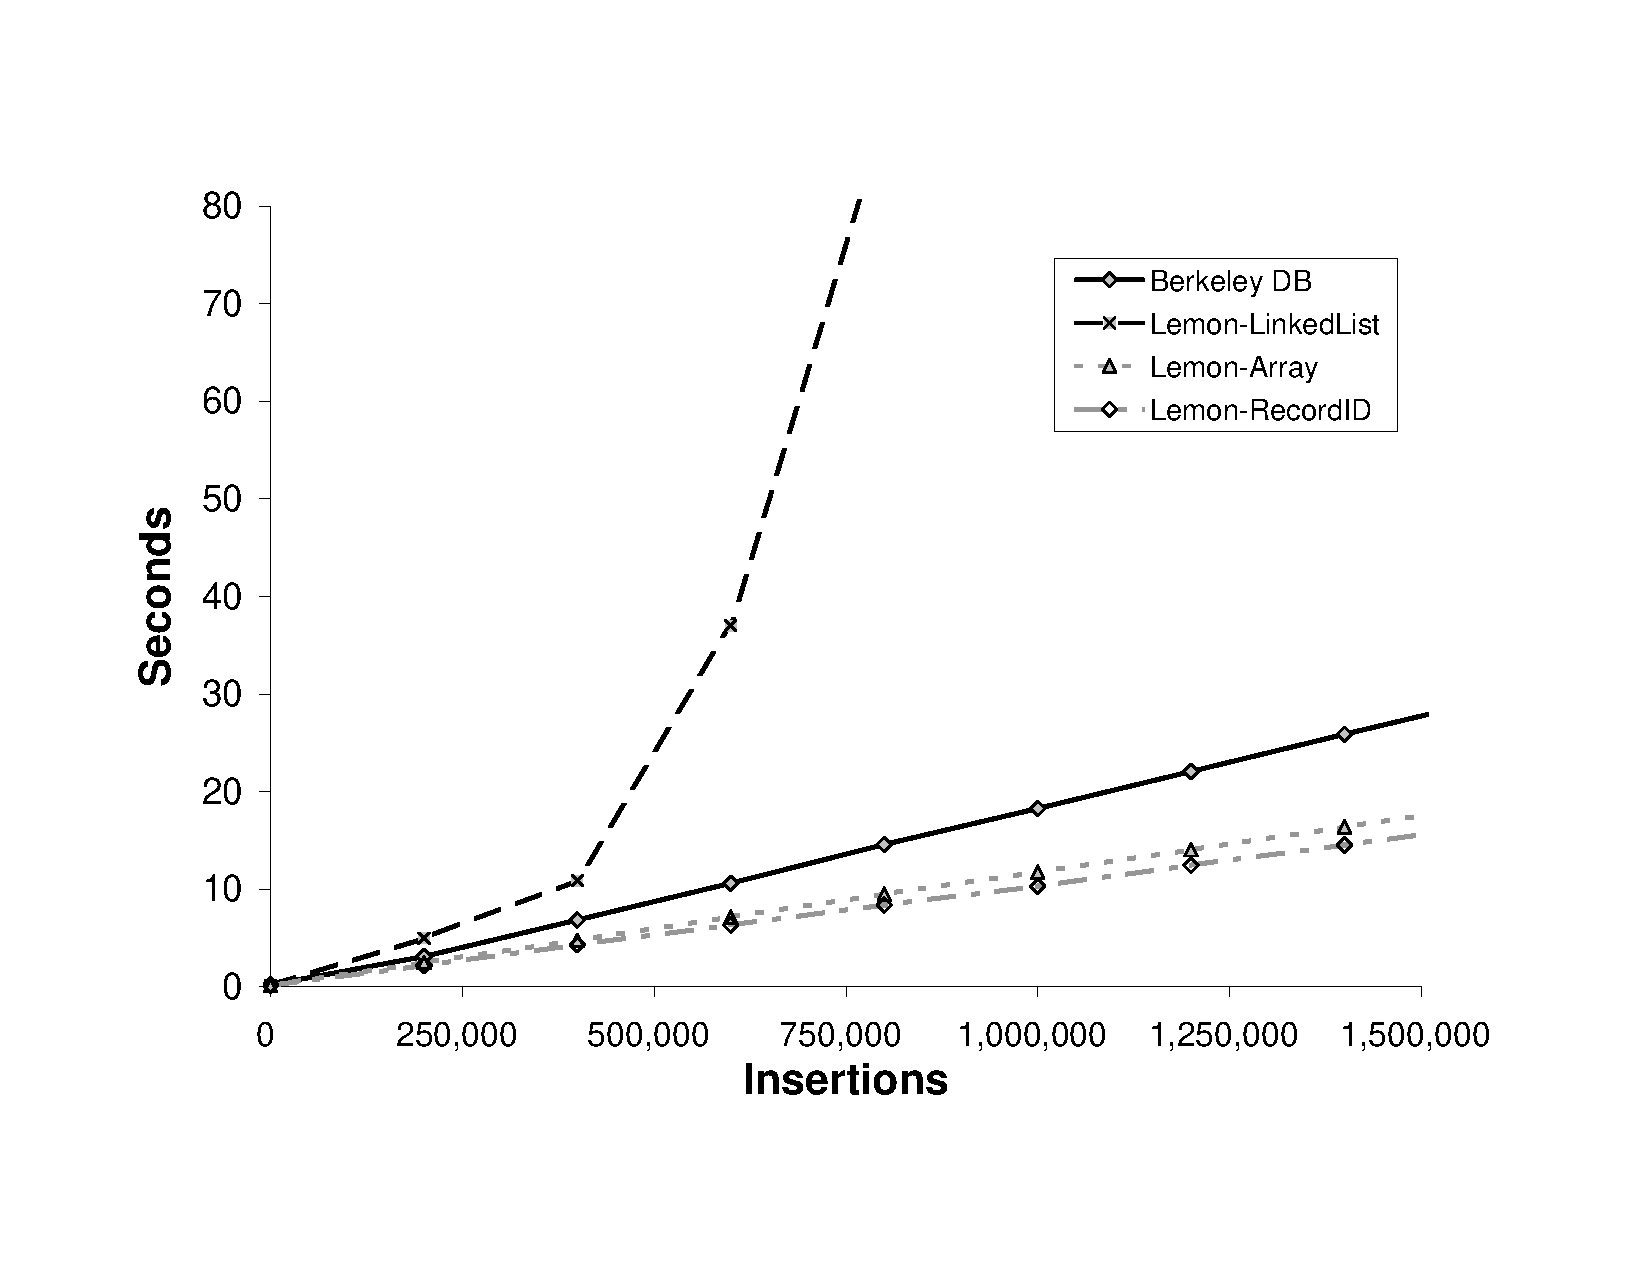
\includegraphics[%
   width=1\columnwidth]{bulk-load-raw.pdf}
\caption{\sf \label{fig:BULK_LOAD} This test measures the raw performance
of the data structures provided by \yad and Berkeley DB.  Since the
test is run as a single transaction, overheads due to synchronous I/O
and logging are minimized.}
\end{figure*}



\subsection{Concurrency}

Given the structures described above, the implementation of a linear
hash table is straightforward.  A linear hash function is used to map
keys to buckets, insertions and deletions are handled by the ArrayList
implementation, and the table can be extended lazily by
transactionally removing items from one bucket and adding them to
another.

Given that the underlying data structures are transactional and a
single lock around the hashtable, this is actually all that is needed
to complete the linear hash table implementation.  Unfortunately, as
we mentioned in Section~\ref{nested-top-actions}, things become a bit
more complex if we allow interleaved transactions.  The solution for
the default hashtable is simply to follow the recipe for Nested
Top Actions, and only lock the whole table during structural changes.
We explore a version with finer-grain locking below.
%This prevents the
%hashtable implementation from fully exploiting multiprocessor
%systems,\footnote{\yad passes regression tests on multiprocessor
%systems.}  but seems to be adequate on single processor machines
%(Figure~\ref{fig:TPS}).
%we describe a finer-grained concurrency mechanism below.

%We have found a simple recipe for converting a non-concurrent data structure into a concurrent one, which involves three steps:
%\begin{enumerate}
%\item Wrap a mutex around each operation, this can be done with a lock
%  manager, or just using pthread mutexes.  This provides isolation.
%\item Define a logical UNDO for each operation (rather than just using
%  the lower-level UNDO in the transactional array).  This is easy for a
%  hash table; e.g. the UNDO for an {\em insert} is {\em remove}.
%\item For mutating operations (not read-only), add a ``begin nested
%  top action'' right after the mutex acquisition, and a ``commit
%  nested top action'' where we release the mutex.
%\end{enumerate}
%
%Note that this scheme prevents multiple threads from accessing the
%hashtable concurrently.  However, it achieves a more important (and
%somewhat unintuitive) goal.  The use of a nested top action protects
%the hashtable against {\em future} modifications by other
%transactions.  Since other transactions may commit even if this
%transaction aborts, we need to make sure that we can safely undo the
%hashtable insertion.  Unfortunately, a future hashtable operation
%could split a hash bucket, or manipulate a bucket overflow list,
%potentially rendering any physical undo information that we could
%record useless.  Therefore, we need to have a logical undo operation
%to protect against this.  However, we could still crash as the
%physical update is taking place, leaving the hashtable in an
%inconsistent state after REDO completes.  Therefore, we need to use
%physical undo until the hashtable operation completes, and then {\em
%switch to} logical undo before any other operation manipulates data we
%just altered.  This is exactly the functionality that a nested top
%action provides.  

%Since a normal hashtable operation is usually fast,
%and this is meant to be a simple hashtable implementation, we simply
%latch the entire hashtable to prevent any other threads from
%manipulating the hashtable until after we switch from physical to
%logical undo.

%\eab{need to explain better why this gives us concurrent
%transactions.. is there a mutex for each record? each bucket?  need to
%explain that the logical undo is really a compensation that undoes the
%insert, but not the structural changes.}

%% To get around
%% this, and to allow multithreaded access to the hashtable, we protect
%% all of the hashtable operations with pthread mutexes. \eab{is this a lock manager, a latch or neither?}  Then, we
%% implement inverse operations for each operation we want to support
%% (this is trivial in the case of the hash table, since ``insert'' is
%% the logical inverse of ``remove.''), then we add calls to begin nested
%% top actions in each of the places where we added a mutex acquisition,
%% and remove the nested top action wherever we release a mutex.  Of
%% course, nested top actions are not necessary for read only operations.

This completes our description of \yad's default hashtable
implementation.  We would like to emphasize the fact that implementing
transactional support and concurrency for this data structure is
straightforward.  The only complications are a) defining a logical UNDO, and b) dealing with fixed-length records.

%, and (other than requiring the design of a logical
%logging format, and the restrictions imposed by fixed length pages) is
%not fundamentally more difficult or than the implementation of normal
%data structures). 

%\eab{this needs updating:} Also, while implementing the hash table, we also
%implemented two generally useful transactional data structures.

%Next we describe some additional optimizations and evaluate the
%performance of our implementations.

\subsection{The Optimized Hashtable}

Our optimized hashtable implementation is optimized for log bandwidth,
only stores fixed-length entries, and exploits a more aggressive
version of nested top actions.

Instead of using nested top actions, the optimized implementation
applies updates in a carefully chosen order that minimizes the extent
to which the on disk representation of the hash table can be
corrupted (Figure~\ref{linkedList}). Before beginning updates, it
writes an UNDO entry that will check and restore the consistency of
the hashtable during recovery, and then invokes the inverse of the
operation that needs to be undone.  This recovery scheme does not
require record-level UNDO information.  Therefore, pre-images of
records do not need to be written to log, saving log bandwidth and
enhancing performance.

Also, since this implementation does not need to support variable-size
entries, it stores the first entry of each bucket in the ArrayList
that represents the bucket list, reducing the number of buffer manager
calls that must be made.  Finally, this implementation caches
the header information in memory, rather than getting it from the buffer manager on each request.

The most important component of \yad for this optimization is \yad's
flexible recovery and logging scheme.  For brevity we only mention
that this hashtable implementation uses bucket-granularity latching;
fine-grain latching is relatively easy in this case since all
operations only affect a few buckets, and buckets have a natural
ordering.


\subsection{Performance}

We ran a number of benchmarks on the two hashtable implementations
mentioned above, and used Berkeley DB for comparison.

%In the future, we hope that improved
%tool support for \yad will allow application developers to easily apply
%sophisticated optimizations to their operations.  Until then, application 
%developers that settle for ``slow'' straightforward implementations of 
%specialized data structures should achieve better performance than would
%be possible by using existing systems that only provide general purpose 
%primitives.

The first test (Figure~\ref{fig:BULK_LOAD}) measures the throughput of
a single long-running
transaction that loads a synthetic data set into the
library.  For comparison, we also provide throughput for many different
\yad operations, BerkeleyDB's DB\_HASH hashtable implementation,
and lower level DB\_RECNO record number based interface.  

Both of \yad's hashtable implementations perform well, but the
optimized implementation is clearly faster.  This is not surprising as
it issues fewer buffer manager requests and writes fewer log entries
than the straightforward implementation.

\eab{missing} With the exception of the page oriented list, we see 
that \yad's other operation implementations also perform well in 
this test.  The page-oriented list implementation is
geared toward preserving the locality of short lists, and we see that
it has quadratic performance in this test.  This is because the list
is traversed each time a new page must be allocated.

%Note that page allocation is relatively infrequent since many entries
%will typically fit on the same page.  In the case of our linear
%hashtable, bucket reorganization ensures that the average occupancy of
%a bucket is less than one.  Buckets that have recently had entries
%added to them will tend to have occupancies greater than or equal to
%one.  As the average occupancy of these buckets drops over time, the
%page oriented list should have the opportunity to allocate space on
%pages that it already occupies.

Since the linear hash table bounds the length of these lists, 
asymptotic behavior of the list is less important than the 
behavior with a bounded number of list entries.  In a separate experiment
not presented here, we compared the implementation of the 
page-oriented linked list to \yad's conventional linked-list 
implementation, and found that the page-oriented list is faster 
when used within the context of our hashtable implementation.

%The NTA (Nested Top Action) version of \yad's hash table is very
%cleanly implemented by making use of existing \yad data structures,
%and is not fundamentally more complex then normal multithreaded code.
%We expect application developers to write code in this style.  

%{\em @todo need to explain why page-oriented list is slower in the
%second chart, but provides better hashtable performance.}

The second test (Figure~\ref{fig:TPS}) measures the two libraries' ability to exploit
concurrent transactions to reduce logging overhead.  Both systems
can service concurrent calls to commit with a single 
synchronous I/O.~\footnote{The multi-threading benchmarks presented 
here were performed using an ext3 file system, as high thread 
concurrency caused Berkeley DB and \yad to behave unpredictably 
when reiserfs was used.  However, \yad's multithreaded throughput was 
significantly better than Berkeley DB's with both filesystems.}


%Because different approaches to this 
%optimization make sense under different circumstances~\cite{findWorkOnThisOrRemoveTheSentence}, this may 
%be another aspect of transactional storage systems where
%application control over a transactional storage policy is 
%desirable.

%\footnote{Although our current implementation does not provide the hooks that 
%would be necessary to alter log scheduling policy, the logger 
%interface is cleanly separated from the rest of \yad.  In fact, 
%the current commit merging policy was implemented in an hour or 
%two, months after the log file implementation was written.  In 
%future work, we would like to explore the possibility of virtualizing 
%more of \yad's internal APIs.  Our choice of C as an implementation 
%language complicates this task somewhat.}

%\rcs{Is the graph for the next paragraph worth the space?}
%\eab{I can combine them onto one graph I think (not 2).}
%
%The final test measures the maximum number of sustainable transactions
%per second for the two libraries.  In these cases, we generate a
%uniform number of transactions per second by spawning a fixed number of
%threads, and varying the number of requests each thread issues per
%second, and report the cumulative density of the distribution of
%response times for each case.
%
%\rcs{analysis / come up with a more sane graph format.}

Finally, we developed a simple load generator which spawns a pool of threads that
generate a fixed number of requests per second.  We then measured
response latency, and found that Berkeley DB and \yad behave
similarly.

In summary, there are a number of primatives that are necessary to
implement custom, high concurrency and low level transactional data
structures.  In order to implement and optimize a hashtable we used a
number of low level APIs that are not supported by other systems.  We
needed to customize page layouts to implement ArrayList.  The page-oriented
list addresses and allocates data with respect to pages in order to
preserve locality.  The hashtable implementation is built upon these two
data structures, and needs to be able to generate custom log entries,
define custom latching/locking semantics, and make use of, or
implement a custom variant of nested top actions.

The fact that our straightforward hashtable is competitive 
with Berkeley DB shows that
straightforward implementations of specialized data structures can 
compete with comparable, highly-tuned, general-purpose implementations.  
Similarly, it seems as though it is not difficult to implement specialized 
data structures that can significantly outperform existing 
general purpose structures.

This finding suggests that it is appropriate for
application developers to consider the development of custom
transactional storage mechanisms when application performance is
important.  The next two sections are devoted to confirming the 
practicality of such mechanisms by applying them to applications 
that suffer from long-standing performance problems with layered 
transactional systems.


%This section uses:
%\begin{enumerate}
%\item{Custom page layouts to implement ArrayList}
%\item{Addresses data by page to preserve locality (contrast w/ other systems..)}
%\item{Custom log formats to implement logical undo}
%\item{Varying levels of latching}
%\item{Nested Top Actions for simple implementation.}
%\item{Bypasses Nested Top Action API to optimize log bandwidth}
%\end{enumerate}


\begin{figure*}
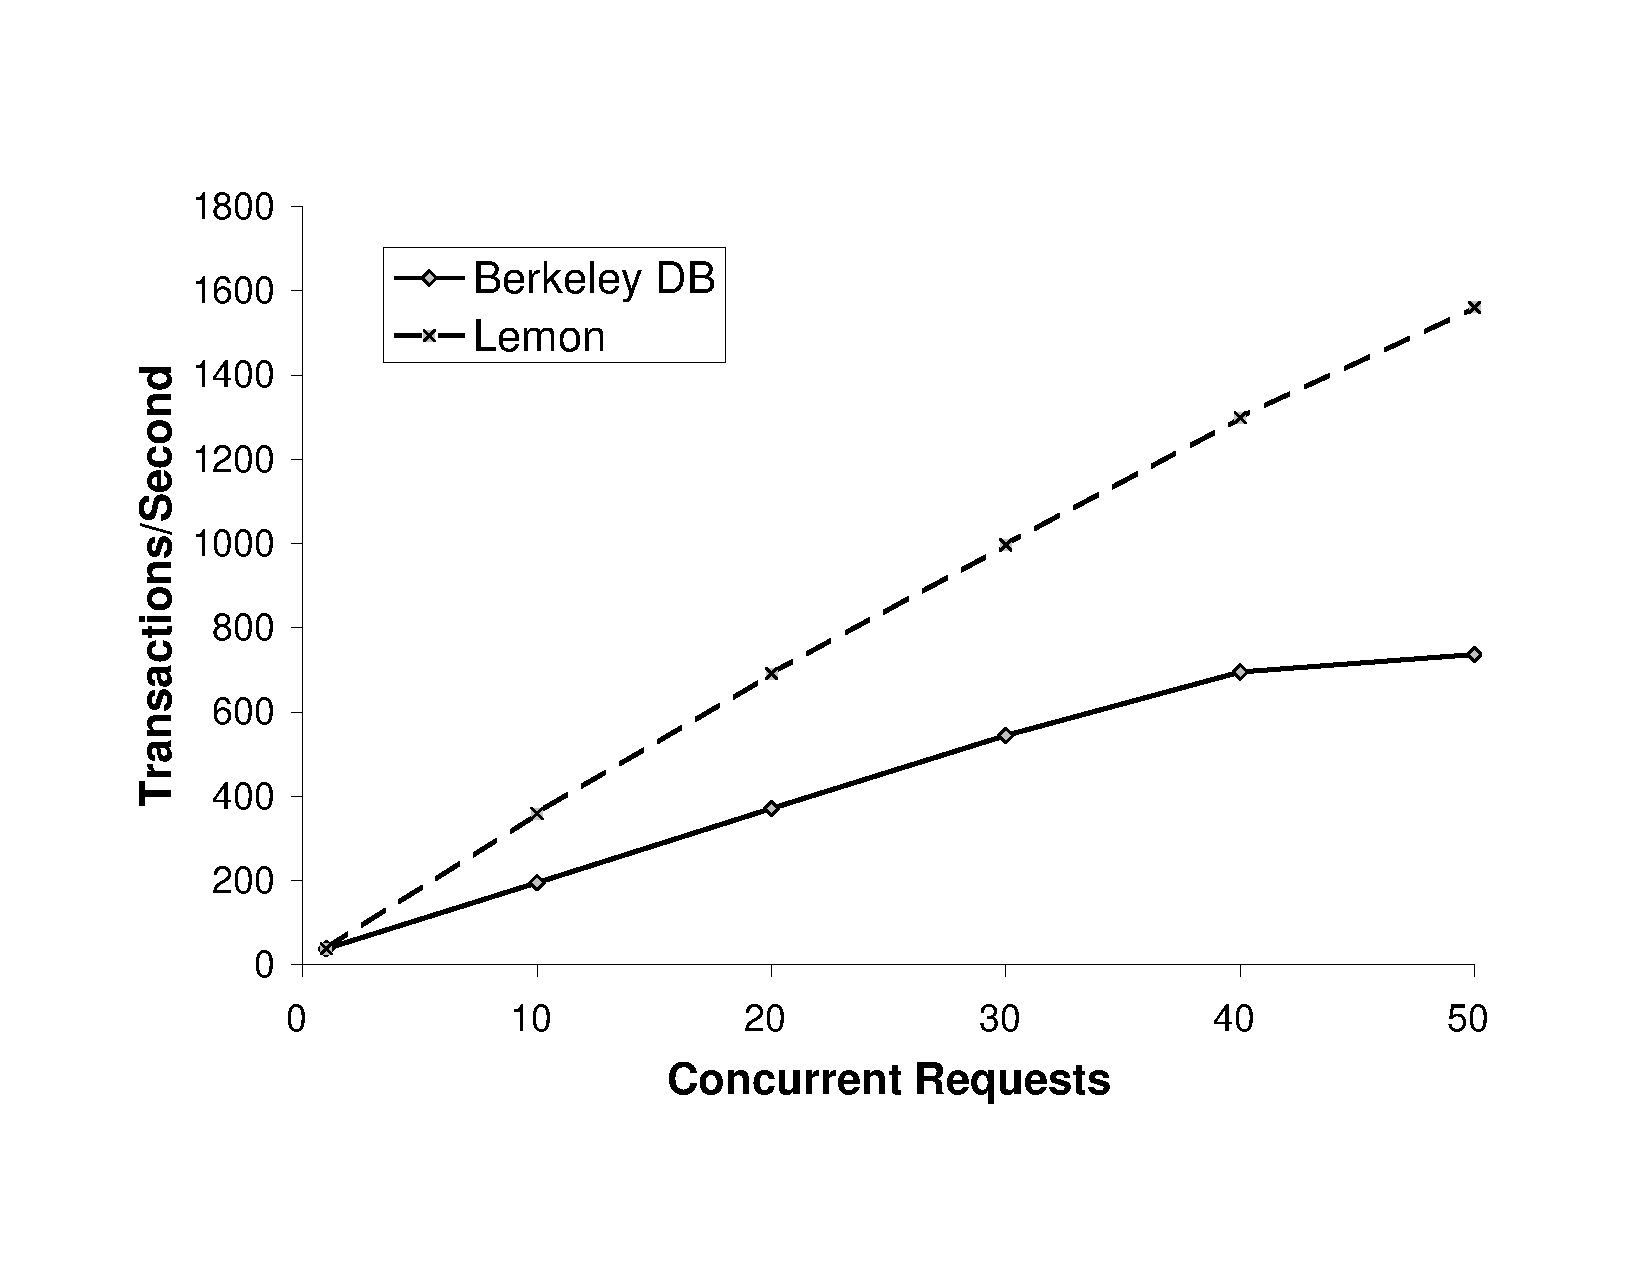
\includegraphics[%
   width=1\columnwidth]{tps-new.pdf}
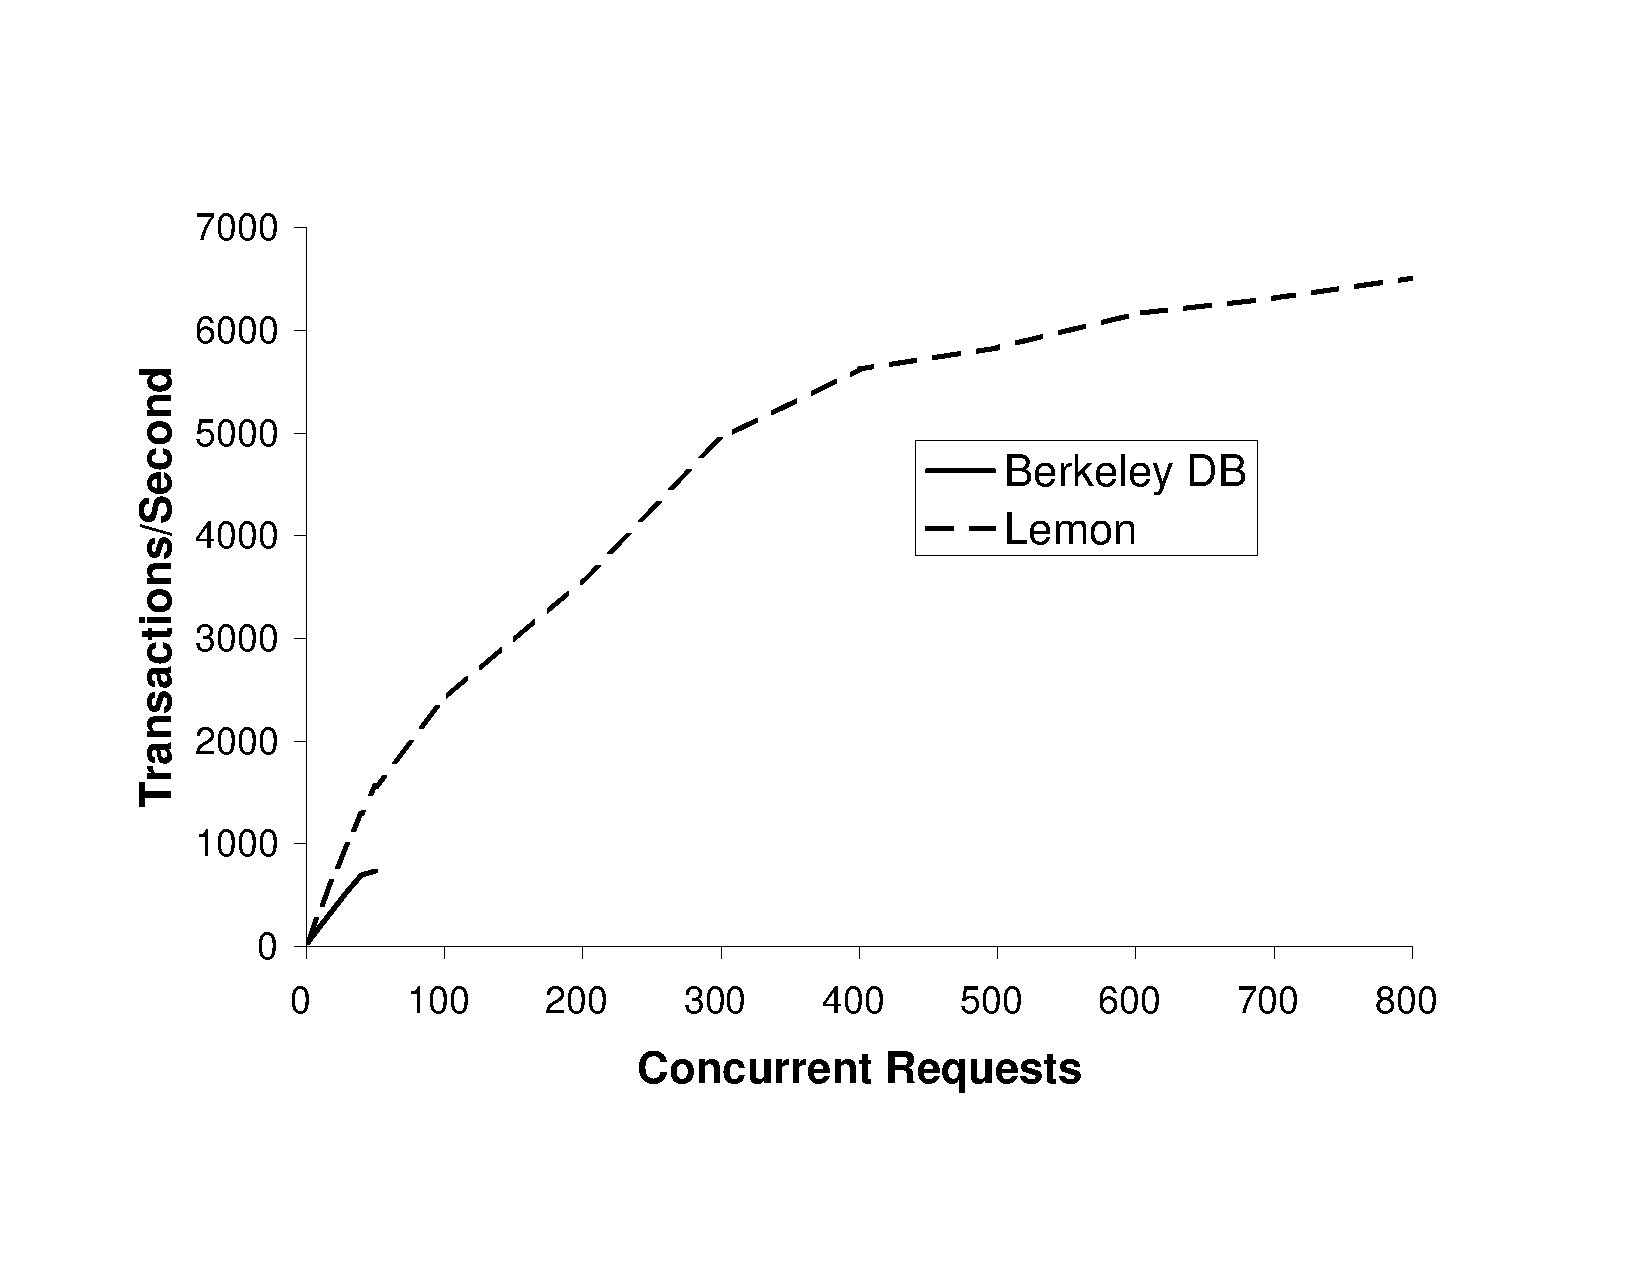
\includegraphics[%
   width=1\columnwidth]{tps-extended.pdf}
\caption{\sf \label{fig:TPS} The logging mechanisms of \yad and Berkeley
DB are able to combine multiple calls to commit() into a single disk 
force, increasing throughput as the number of concurrent transactions 
grows.  A problem with our testing environment prevented us from 
scaling Berkeley DB past 50 threads.
} 
\end{figure*}

\section{Object Serialization}
\label{OASYS}

Object serialization performance is extremely important in modern web
application systems such as Enterprise Java Beans.  Object
serialization is also a convenient way of adding persistent storage to
an existing application without developing an explicit file format or
dealing with low-level I/O interfaces.

A simple object serialization scheme would bulk-write and bulk-read
sets of application objects to an OS file.  These simple
schemes suffer from high read and write latency, and do not handle
small updates well.  More sophisticated schemes store each object in a
separate, randomly accessible record, such as a database  or
 Berkeley DB record.  These schemes allow for fast single-object reads and writes, and are typically the solutions used by
application servers.

However, one drawback of many such schemes is that any update requires
a full serialization of the entire object. In some application
scenarios this can be extremely inefficient as it may be the case
that only a single field from a large complex object has been
modified.

Furthermore, most of these schemes ``double cache'' object
data.  Typically, the application maintains a set of in-memory
objects in their unserialized form, so they can be accessed with low latency.
The backing store also
maintains a separate in-memory buffer pool with the serialized versions of
some objects, as a cache of the on-disk data representation.
Accesses to objects that are only present in the serialized buffers
pool incur significant latency, as they must be unmarshalled (deserialized)
before the application may access them.  
There may even be a third copy of this data resident in the filesystem 
buffer cache, accesses to which incur latency of both system call overhead and
the unmarshalling cost.

To maximize performance we want to maximize the size of the in-memory object cache.
However, naively constraining the size of the data store's buffer pool
causes performance degradation. Most transactional layers 
(including ARIES) must read a page
into memory to service a write request to the page; if the buffer pool
is too small, these operations trigger potentially random disk I/O. 
This removes the primary
advantage of write ahead logging, which is to ensure application data
durability with mostly sequential disk I/O.

In summary, this system architecture (though commonly
deployed~\cite{ejb,ordbms,jdo,...}) is fundamentally
flawed.  In order to access objects quickly, the application must keep
its working set in cache.  Yet in order to efficiently service write 
requests, the
transactional layer must store a copy of serialized objects
in memory or resort to random I/O.  
Thus, any given working set size requires roughly double the system
memory to achieve good performance.

\subsection{\yad Optimizations}

\label{version-pages}

\yad's architecture allows us to apply two interesting optimizations
to object serialization.  First, since \yad supports
custom log entries, it is trivial to have it store deltas to
the log instead of writing the entire object during an update.
Such an optimization would be difficult to achieve with Berkeley DB 
since the only diff-based mechanism it supports requires changes to 
span contiguous regions of a record, which is not necessarily the case for arbitrary
object updates.
In a database server context, this type of optimization can be
supported if the fields of the object are broken into database table
columns. and a SQL update query only modifies a subset of the fields. 
However, as we have seen in some preliminary evaluation, 
the overheads associated with a SQL based interface outweigh the
advantages of this optimization.  To avoid RPC costs, we ran the 
benchmark using libmysqld, which bypasses RPC costs by linking MySQL 
into an application binary.  We used an InnoDB table, which seemed 
to perform better than tables backed by Berkeley DB.  Still, MySQL 
was significantly slower then native Berkeley DB.  If we do not link 
MySQL the MySQL server into the application binary then the cost of local 
interprocess communication dominates the test, causing the benchmark to 
take too long to be reported here.

%% \footnote{It is unclear if
%% this optimization would outweigh the overheads associated with an SQL
%% based interface.  Depending on the database server, it may be
%% necessary to issue a SQL update query that only updates a subset of a
%% tuple's fields in order to generate a diff-based log entry.  Doing so
%% would preclude the use of prepared statements, or would require a large
%% number of prepared statements to be maintained by the DBMS. We plan to
%% investigate the overheads of SQL in this context in the future.}

%  If IPC or 
%the network is being used to communicate with the DBMS, then it is very
%likely that a separate prepared statement for each type of diff that the 
%application produces would be necessary for optimal performance.  
%Otherwise, the database client library would have to determine which 
%fields of a tuple changed since the last time the tuple was fetched 
%from the server, and doing this would require a large amount of state 
%to be maintained.

% @todo WRITE SQL OASYS BENCHMARK!!

The second optimization is a bit more sophisticated, but still easy to
implement in \yad.  This optimization allows us to drastically limit
the size of the
\yad buffer cache, yet still achieve good performance.
We do not believe that it would be possible to
achieve using existing relational database systems or with Berkeley DB.  

The basic idea of this optimization is to postpone expensive
operations that update the page file for frequently modified objects,
relying on some support from the application's object cache
to maintain transactional semantics.

To implement this, we added two custom \yad operations. The
{\tt``update()''} operation is called when an object is modified and
still exists in the object cache. This causes a log entry to be
written, but does not update the page file. The fact that the modified
object still resides in the object cache guarantees that the (now stale)
records will not be read from the page file. The {\tt ``flush()''}
operation is called whenever a modified object is evicted from the
cache. This operation updates the object in the buffer pool (and
therefore the page file), likely incurring the cost of both a disk {\em
read} to pull in the page, and a {\em write} to evict another page
from the relative small buffer pool.  However, since popular 
objects tend to remain in the object cache, multiple update
modifications will incur relatively inexpensive log additions,
and are only coalesced into a single modification to the page file
when the object is flushed from cache.

\yad provides a several options  to handle UNDO records in the context
of object serialization. The first is to use a single transaction for
each object modification, avoiding the cost of generating or logging
any UNDO records. The second option is to assume that the
application will provide a custom UNDO for the delta, 
which requires a log entry for each update, 
but still avoids the need to read or update the page
file.

The third option is to relax the atomicity requirements for a set of
object updates, and again avoid generating any UNDO records. This
assumes that the application cannot abort individual updates, 
and is willing to
accept that some prefix of logged but uncommitted updates may 
be applied to the page
file after recovery. These ``transactions'' would still be durable
after commit(), as it would force the log to disk. 
For the benchmarks below, we
use this approach, as it is the most aggressive and is
not supported by any other general purpose transactional 
storage system that we know of.

\subsection{Recovery and Log Truncation}

An observant reader may have noticed a subtle problem with this
scheme.  More than one object may reside on a page, and we do not
constrain the order in which the cache calls flush() to evict objects.
Recall that the version of the LSN on the page implies that all
updates {\em up to} and including the page LSN have been applied.
Nothing stops our current scheme from breaking this invariant.  

This where we use the versioned-record page layout. This layout adds a
``record sequence number'' (RSN) for each record, which subsumes the
page LSN.  Instead of the invariant that the page LSN implies that all
earlier {\em page} updates have been applied, we enforce that all
previous {\em record} updates have been applied.  One way to think about
this optimization is that it removes the head-of-line blocking implied
by the page LSN so that unrelated updates remain independent.

Recovery work essentially the same as before, except that we need to
use RSNs to calculate the earliest allowed point for log truncation
(so as to not lose an older record update).  In the implementation, we
also periodically flush the object cache to move the truncation point
forward, but this is not required.

%% We have two solutions to this problem.  One solution is to
%% implement a cache eviction policy that respects the ordering of object
%% updates on a per-page basis.  
%% However, this approach would impose an unnatural restriction on the
%% cache replacement policy, and would likely suffer from performance
%% impacts resulting from the (arbitrary) manner in which \yad allocates
%% objects to pages.

%% The second solution is to 
%% force \yad to ignore the page LSN values when considering
%% special {\tt update()} log entries during the REDO phase of recovery.  This
%% forces \yad to re-apply the diffs in the same order in which the application
%% generated them.  This works as intended because we use an
%% idempotent diff format that will produce the correct result even if we
%% start with a copy of the object that is newer than the first diff that
%% we apply.

%% To avoid needing to replay the entire log on recovery, we add a custom
%% checkpointing algorithm that interacts with the page cache.  
%% To produce a
%% fuzzy checkpoint, we simply iterate over the object pool, calculating
%% the minimum LSN of the {\em first} call to update() on any object in
%% the pool (that has not yet called flush()). 
%% We can then invoke a normal ARIES checkpoint with the restriction
%% that the log is not truncated past the minimum LSN encountered in the
%% object pool.\footnote{We do not yet enforce this checkpoint limitation.}
%% A background process that calls flush() for all objects in the cache
%% allows efficient log truncation without blocking any high-priority 
%% operations.

\begin{figure*}[t!]
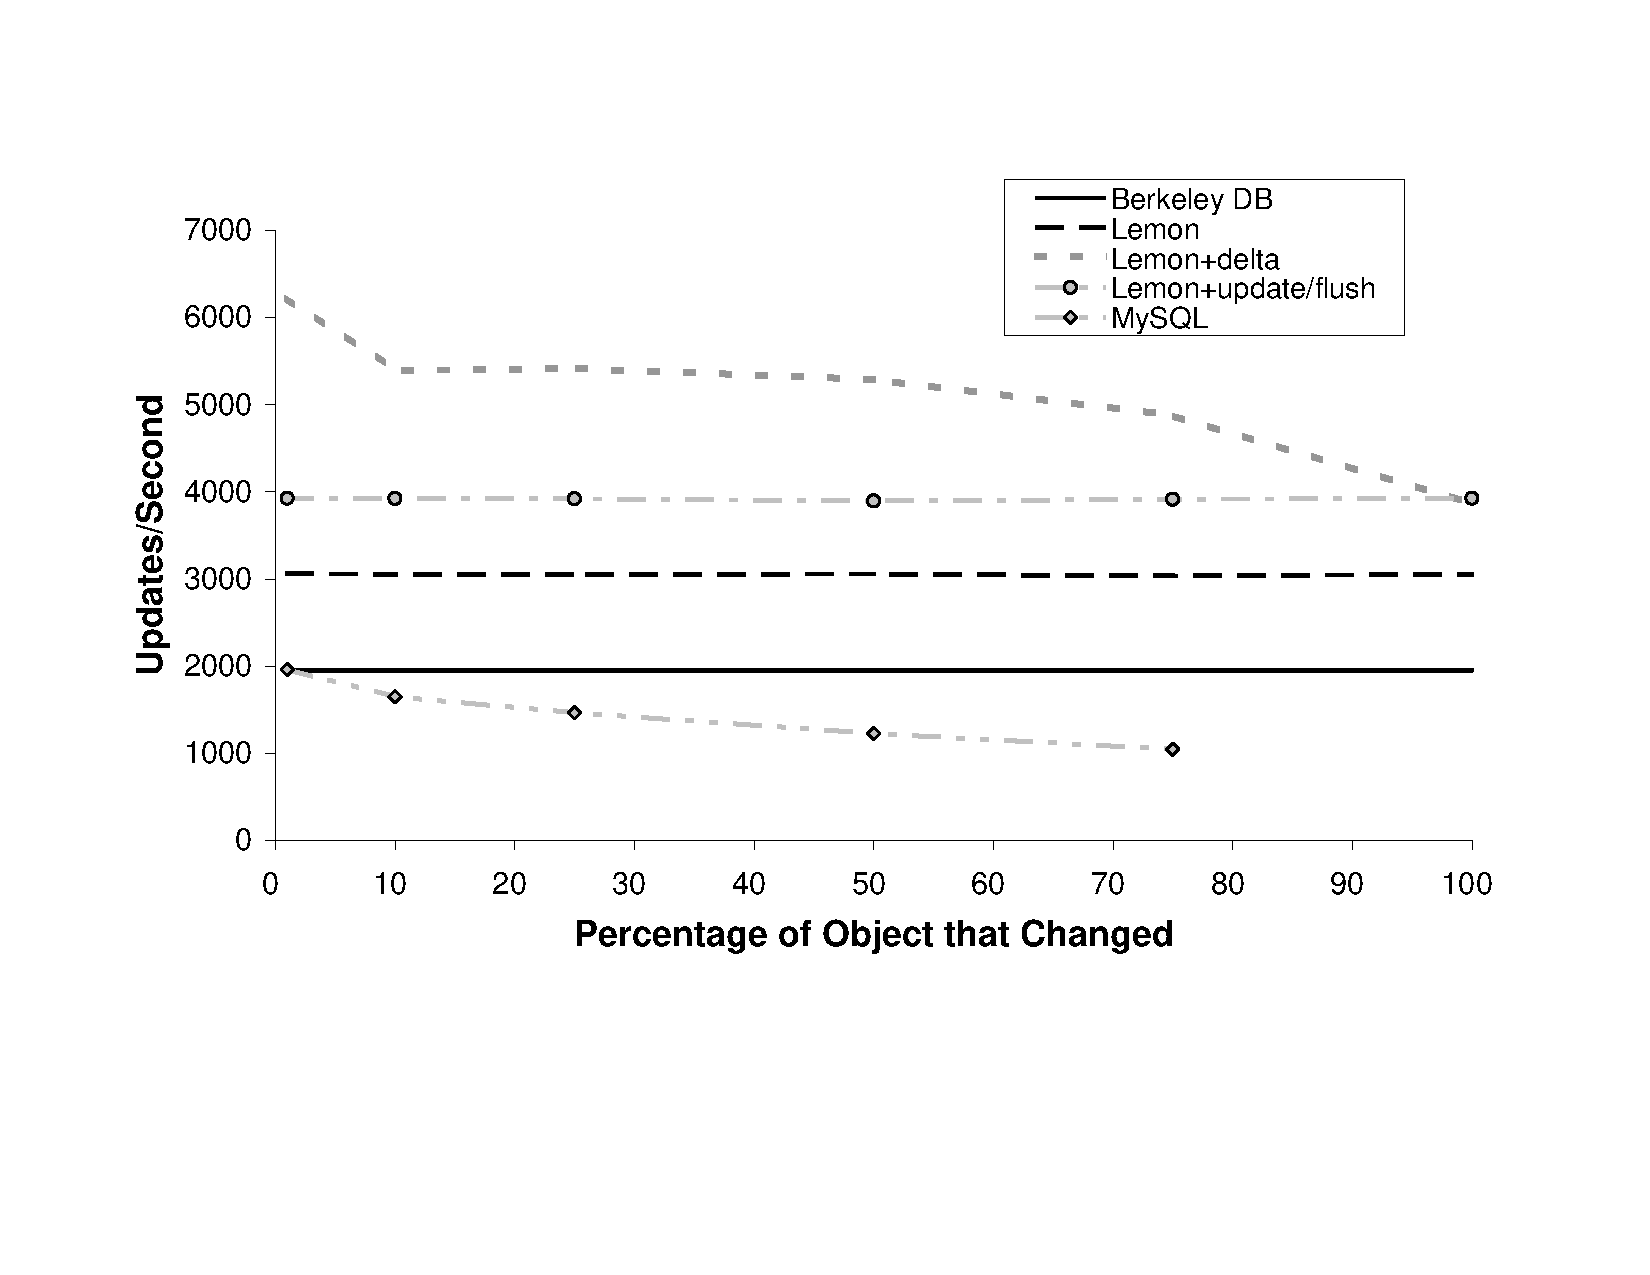
\includegraphics[width=3.3in]{object-diff.pdf}
\hspace{.3in}
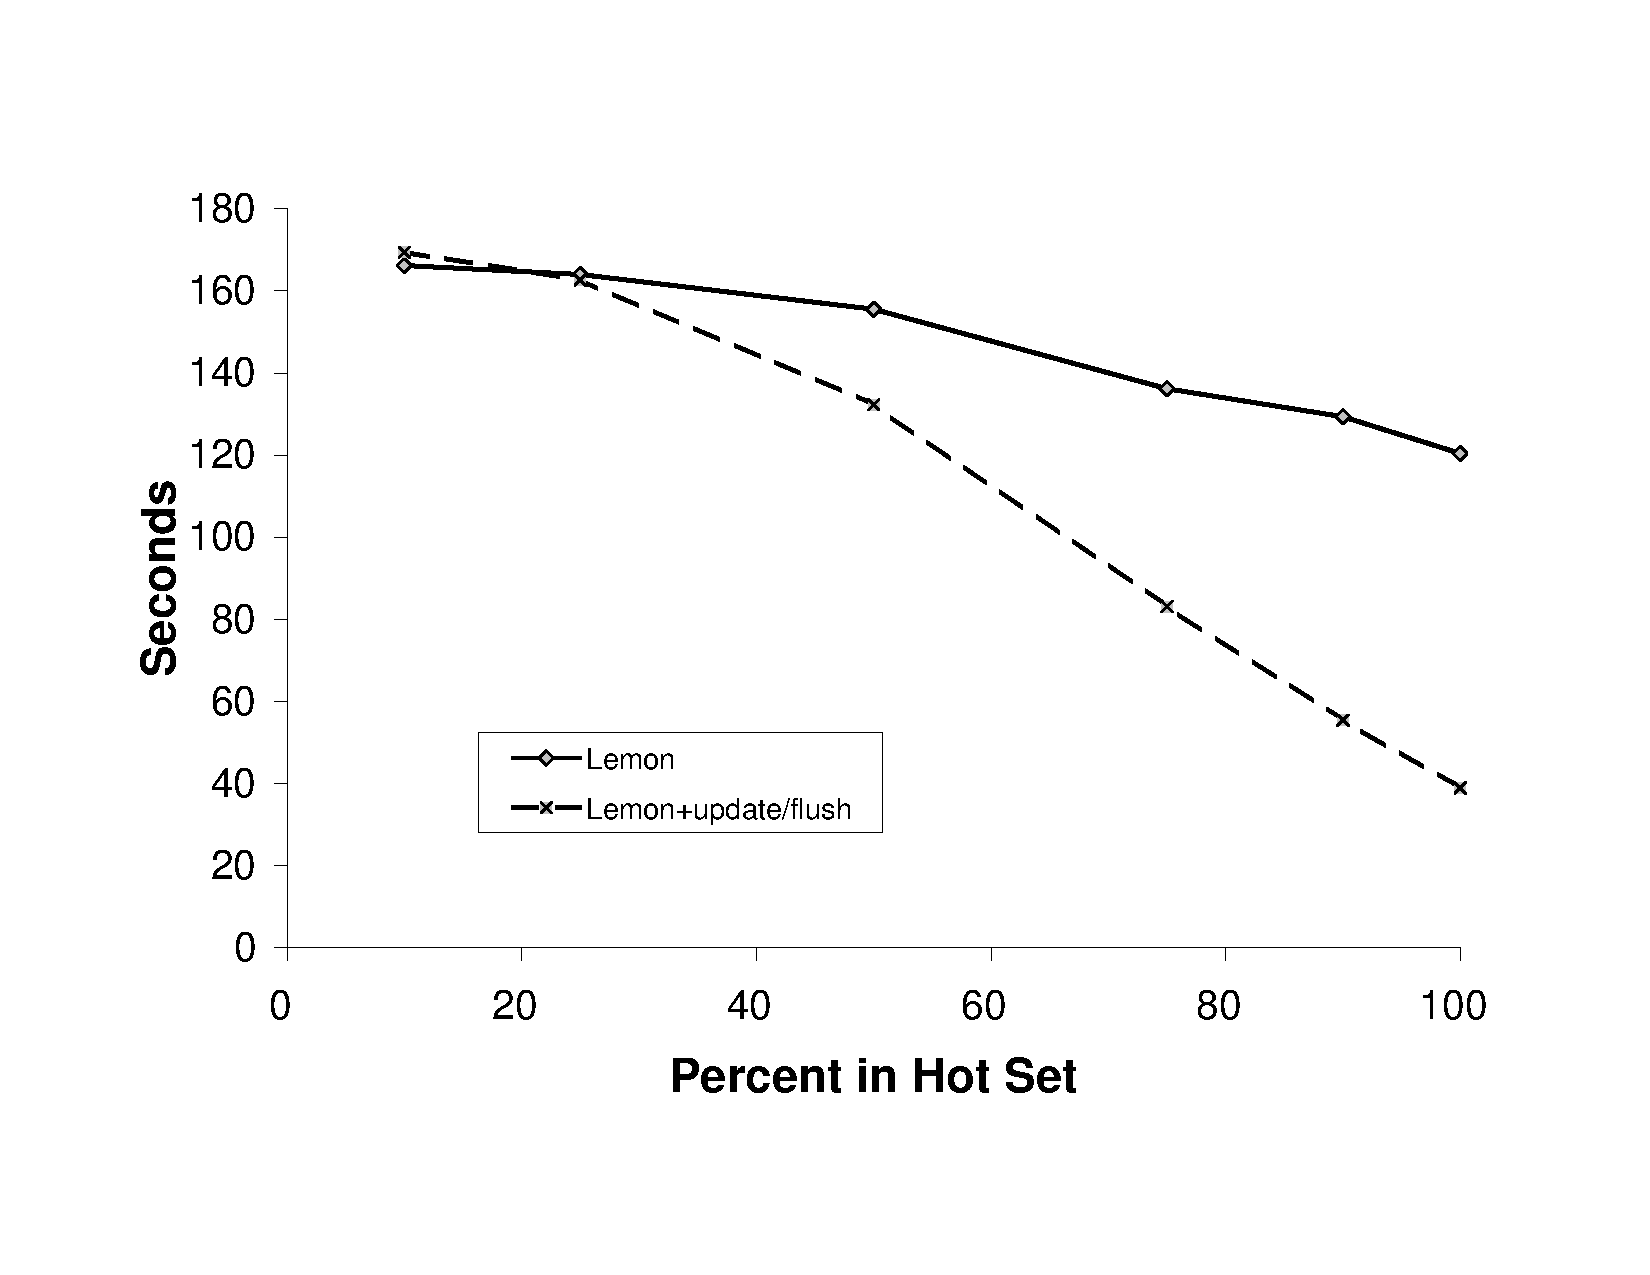
\includegraphics[width=3.3in]{mem-pressure.pdf}
\caption{\sf \label{fig:OASYS}
\yad optimizations for object
serialization. The first graph shows the effect of the two \yad
optimizations as a function of the portion of the object that is being
modified. The second graph focuses on the 
benefits of the update/flush optimization in cases of system
memory pressure.}
\end{figure*}

\subsection{Evaluation}

We implemented a \yad plugin for \oasys, a C++ object serialization
library that can use various object serialization backends. 
We set up an experiment in which objects are randomly
retrieved from the cache according to a hot-set distribution\footnote{In
an example hot-set distribution, 10\% of the objects (the hot set size) are
selected 90\% of the time (the hot set probability).} 
and then have certain fields modified and
updated into the data store. For all experiments, the number of objects
is fixed at 5,000, the
hot set is set to 10\% of the objects, the object cache is set to
double the size of the hot set, we update 100 objects per
transaction, and all experiments were run with identical random seeds 
for all configurations.

The first graph in Figure \ref{fig:OASYS} shows the update rate as we
vary the fraction of the object that is modified by each update for
Berkeley DB, unmodified \yad, \yad with the update/flush optimization,
and \yad with both the update/flush optimization and diff based log
records.
The graph confirms that the savings in log bandwidth and
buffer pool overhead by both \yad optimizations 
outweighs the overhead of the operations, especially when only a small
fraction of the object is modified.
In the most extreme case, when
only one integer field from a ~1KB object is modified, the fully
optimized \yad correspond to a twofold speedup over the unoptimized
\yad.

In all cases, the update rate for mysql\footnote{We ran mysql using
InnoDB for the table engine, as it is the fastest engine that provides
similar durability to \yad. For this test, we also linked directly
with the mysqld daemon library, bypassing the RPC layer. In
experiments that used the RPC layer, test completion times were orders
of magnitude slower.} is slower than Berkeley DB,
which is slower than any of the \yad variants. This performance
difference is in line with those observed in Section
\ref{sub:Linear-Hash-Table}. We also see the increased overhead due to
the SQL processing for the mysql implementation, although we note that
a SQL variant of the diff-based optimization also provides performance
benefits.

In the second graph, we constrained the \yad buffer pool size to be a
small fraction of the size of the object cache, and bypass the filesystem
buffer cache via the O\_DIRECT option. The goal of this experiment is to
focus on the benefits of the update/flush optimization in a simulated
scenario of memory pressure. From this graph, we see that as the percentage of
requests that are serviced by the cache increases, the
performance of the optimized \yad dramatically increases.
This result supports the hypothesis of the optimization, and
shows that by leveraging the object cache, we can reduce the load on
the page file and therefore the size of the buffer pool.

The operations required for these
two optimizations required a mere 150 lines of C code, including
whitespace, comments and boilerplate function registrations.  Although
the reasoning required to ensure the correctness of this code is
complex, the simplicity of the implementation is encouraging.

In addition to the hashtable, which is required by \oasys's API, this
section made use of custom log formats and semantics to reduce log
bandwidth and page file usage.  Berkeley DB supports a similar
partial update mechanism, but it only
supports range updates and does not map naturally to \oasys's data
model.  In contrast, our \yad extension simply makes upcalls
into the object serialization layer during recovery to ensure that the
compact, object-specific diffs that \oasys produces are correctly
applied.  The custom log format, when combined with direct access to
the page file and buffer pool, drastically reduces disk and memory usage
for write intensive loads. A simple extension to our recovery algorithm makes it
easy to implement other similar optimizations in the future.

%This section uses:
%
%\begin{enumerate}
%\item{Custom log formats to implement diff based updates}
%\item{Custom log semantics to reduce log bandwidth and page file usage}
%\item{Direct page file access to reduce page file usage}
%\item{Custom recovery and checkpointing semantics to maintain correctness}
%\end{enumerate}

\section{Graph Traversal\label{TransClos}}

Database servers (and most transactional storage systems) are not
designed to handle large graph structures well.  Typically, each edge
traversal will involve an index lookup, and worse, since most systems
do not provide information about the physical layout of the data that
they store, it is not straightforward to implement graph algorithms in
a way that exploits on disk locality.  In this section, we describe an
efficient representation of graph data using \yad's primitives, and
present an optimization that introduces locality into random disk
requests by reordering invocations of wrapper functions.

\subsection {Data Representation}

For simplicity, we represent graph nodes as
fixed-length records.  The Array List from our linear hash table
implementation (Section~\ref{sub:Linear-Hash-Table}) provides access to an
array of such records with performance that is competitive with native
recordid accesses, so we use an ArrayList to store the records.  We
could have opted for a slightly more efficient representation by
implementing a fixed length array structure, but doing so seems to be
overkill for our purposes.  The nodes themselves are stored as an
array of integers of length one greater than their out-degree. The
extra int is used to hold information about the node.  (In our case,
it is simply a set to a constant value by a graph traversal.)

We implement a ``naive'' graph traversal algorithm that uses depth-first search to find all nodes that are reachable from node zero.
This algorithm (predictably) consumes a large amount of memory, as
nothing stops it from placing the entire graph on its stack.  

For the purposes of this section, which focuses on page access
locality, we ignore the amount of memory utilization used to store
stacks and work lists, as they can vary greatly from application to
application, but we note that the memory utilization of the simple
depth-first search algorithm is certainly no better than the algorithm
presented in the next section.

Also, for simplicity, we do not apply any of the optimizations in
Section~\ref{OASYS}.  This allows our performance comparison to
 measure only the optimization presented here.

\subsection {Request Reordering for Locality}

General graph structures may have no intrinsic locality.  If such a
graph is too large to fit into memory, basic graph operations such as
edge traversal become very expensive, which makes many algorithms over
these structures intractable in practice.  In this section, we
describe how \yad's primitives provide a natural way to introduce
physical locality into a sequence of such requests.  These primitives
are general and support a wide class of optimizations, which we discuss
before presenting an evaluation.

\yad's wrapper functions translate high-level (logical) application
requests into lower level (physiological) log entries.  These
physiological log entries generally include a logical UNDO,
(Section~\ref{nested-top-actions}) that invokes the logical
inverse of the application request.  Since the logical inverse of most
application request is another application request, we can {\em reuse} our
logging format and wrapper functions to implement a purely logical log.

\begin{figure}
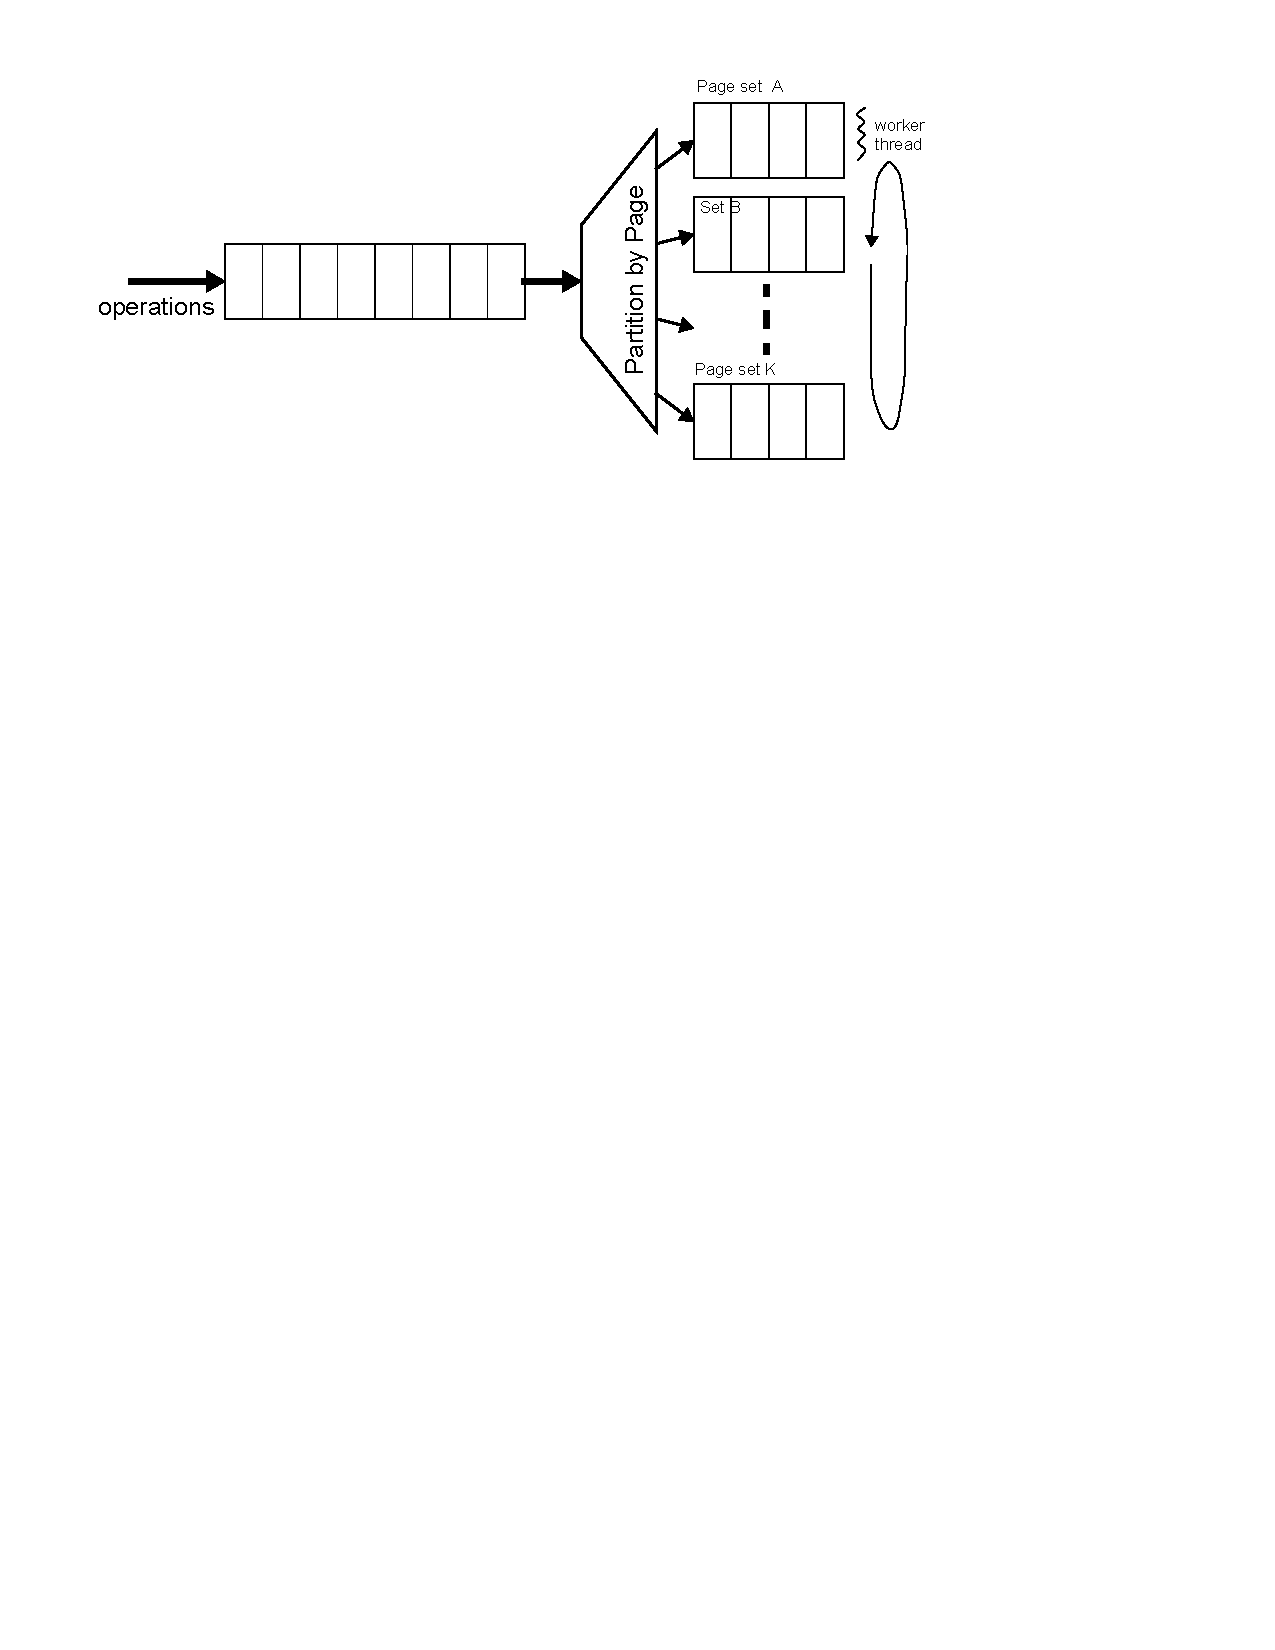
\includegraphics[width=1\columnwidth]{graph-traversal.pdf}
\caption{\sf\label{fig:multiplexor} Because pages are independent, we can reorder requests among different pages. Using a log demultiplexer, we can partition requests into indepedent queues that can then be handled in any order, which can improve locality and simplify log merging.}
\end{figure}

For our graph traversal algorithm we use a {\em log demultiplexer},
shown in Figure~\ref{fig:multiplexor} to route entries from a single
log into many sub-logs according to page number.  This is easy to do
with the Array List representation that we chose for our graph, since
it provides a function that maps from
array index to a $(page, slot, size)$ triple.

The logical log allows us to insert log entries that are independent
of the physical location of their data.  However, we are
interested in exploiting the commutativity of the graph traversal
operation, and saving the logical offset would not provide us with any
obvious benefit.  Therefore, we place use page numbers for partitioning.

We considered a number of multiplexing policies and present two
particularly interesting ones here.  The first divides the page file
up into equally sized contiguous regions, which enables locality.  The second takes the hash
of the page's offset in the file, which enables load balancing.
%  The second policy is interesting
%because it reduces the effect of locality (or lack thereof) between
%the pages that store the graph, while the first better exploits any
%locality intrinsic to the graph's layout on disk.

Requests are continuously consumed by a process that empties each of
the multiplexer's output queues one at a time.  Instead of following
graph edges immediately, the targets of edges leaving each node are
simply pushed into the multiplexer's input queue.  The number of
multiplexer output queues is chosen so that each queue addresses a
subset of the page file that can fit into cache, ensuring locality.  When the
multiplexer's queues contain no more entries, the traversal is
complete.  

Although this algorithm may seem complex, it is essentially just a
queue-based breadth-first search implementation, except that the queue
reorders requests in a way that attempts to establish and maintain
disk locality.  This kind of log manipulation is very powerful, and
could also be used for parallelism with load balancing (using a hash
of the page number) and log-merging optimizations
(e.g. LRVM~\cite{LRVM}),

%% \rcs{ This belongs in future work....}

%% The purely logical log has some interesting properties.  It can be
%% {\em page file independent} as all information expressed within it is
%% expressed in application terms instead of in terms of internal
%% representations.  This means the log entry could be sent over the
%% network and applied on a different system, providing a simple
%% generalization of log based replication schemes.

%% While in transit, various transformations could be applied.  LRVM's
%% log merging optimizations~\cite{LRVM} are one such possibility.
%% Replication and partitioning schemes are another possibility.  If a
%% lock manager is not in use and a consistent order is imposed upon
%% requests,\footnote{and we assume all failures are recoverable or
%% masked with redundancy} then we can remove replicas' ability to
%% unilaterally abort transactions, allowing requests to commit as they
%% propagate through the network, but before actually being applied to
%% page files.

%However, most of \yad's current functionality focuses upon the single
%node case, so we decided to choose a single node optimization for this
%section, and leave networked logical logging to future work.  To this
%end, we implemented a log multiplexing primitive which splits log
%entries into multiple logs according to the value returned by a
%callback function. (Figure~\ref{fig:mux})

\subsection {Performance Evaluation}

\begin{figure}[t]
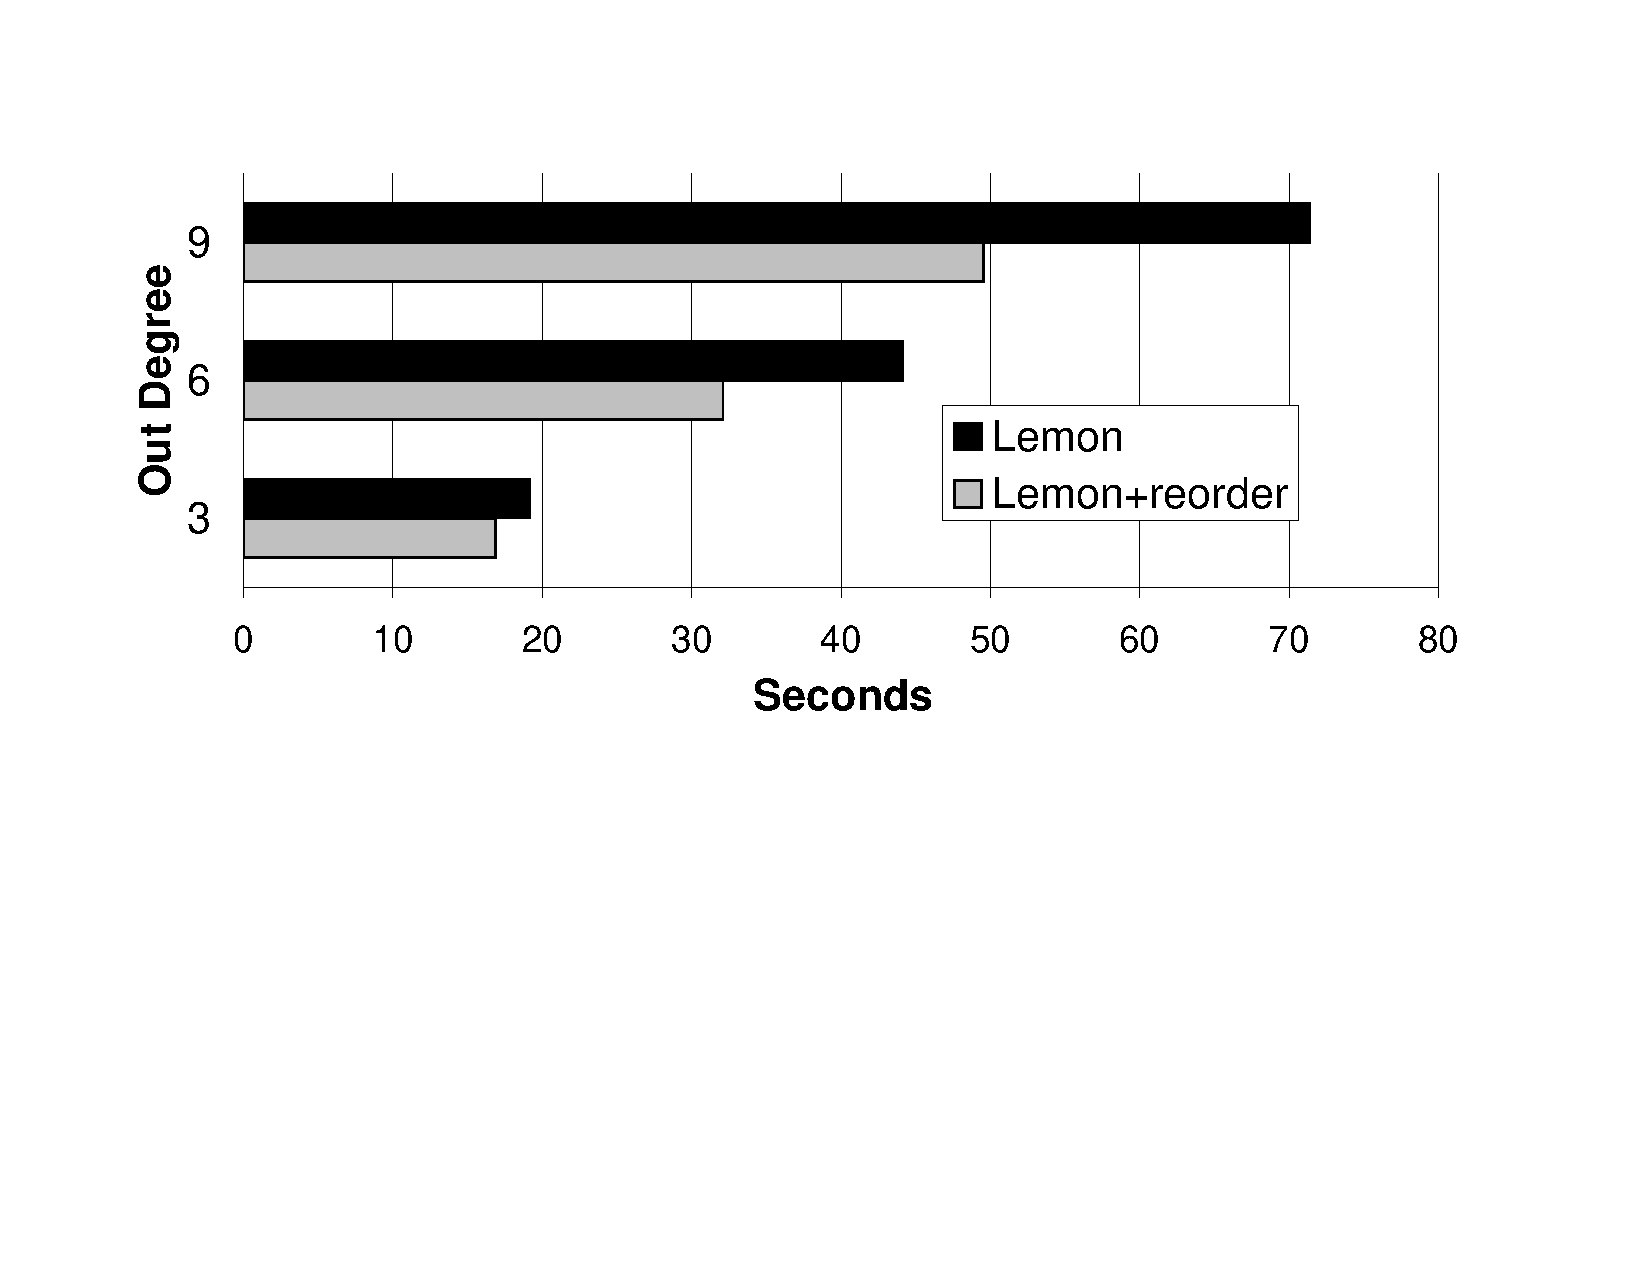
\includegraphics[width=3.3in]{oo7.pdf}
\caption{\sf\label{fig:oo7} oo7...}
\end{figure}

\begin{figure}[t]
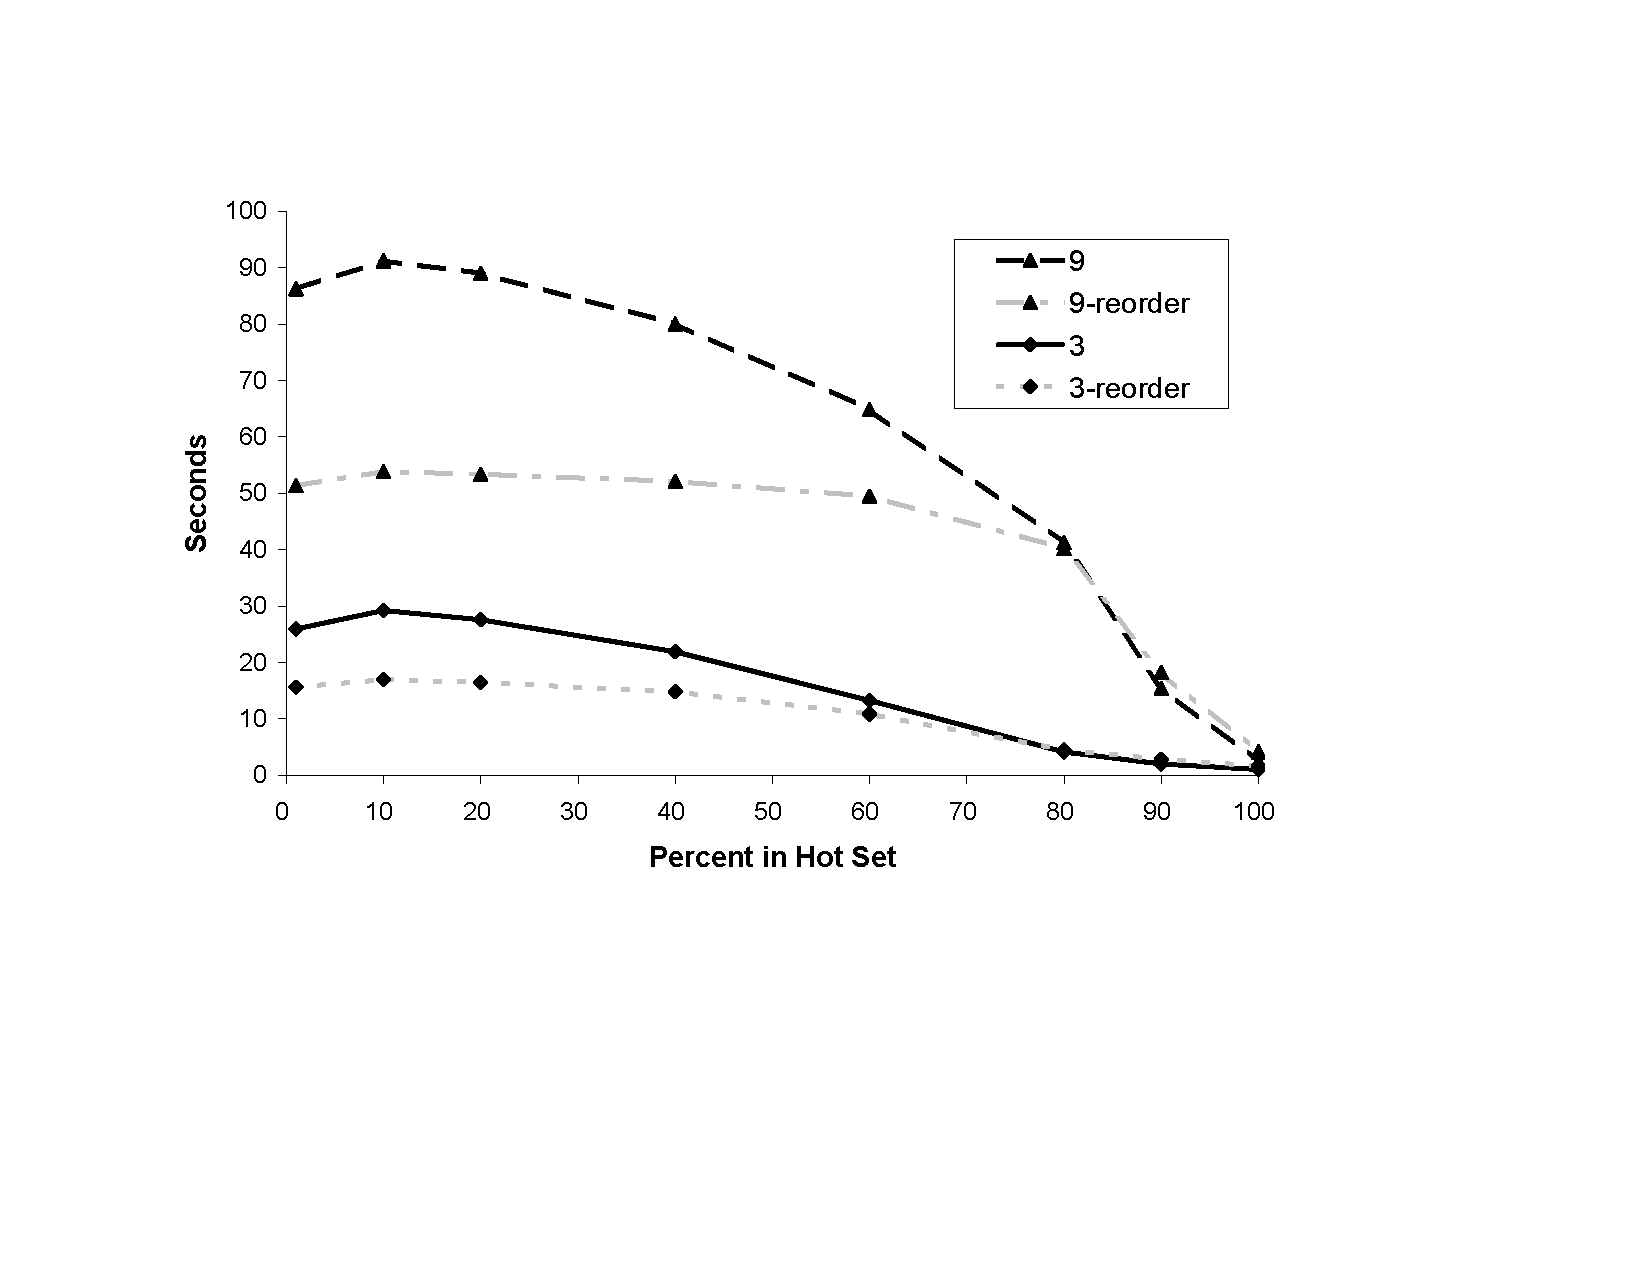
\includegraphics[width=3.3in]{trans-closure-hotset.pdf}
\caption{\sf\label{fig:hotGraph} hotset...}
\end{figure}

We loosely base the graphs for this test on the graphs used by the oo7
benchmark~\cite{oo7}.  For the test, we hard code the out-degree of
graph nodes to 3, 6 and 9 and use a directed graph.  The oo7 benchmark
constructs graphs by first connecting nodes together into a ring.  It
then randomly adds edges between the nodes until the desired out-degree
is obtained.  This structure ensures graph connectivity.  If the nodes
are laid out in ring order on disk, it also ensures that one edge
from each node has good locality, while the others generally have poor
locality.  The results for this test are presented in
Figure~\ref{oo7}, and we can see that the request reordering algorithm
helps performance.  We re-ran the test without the ring edges, and (in
line with our next set of results) found that the reordering algorithm
also helped in that case.

In order to get a better feel for the effect of graph locality on the
two traversal algorithms we extend the idea of a hot set to graph
generation.  Each node has a distinct hot set which includes the 10\%
of the nodes that are closest to it in ring order.  The remaining
nodes are in the cold set.  We use random edges instead of ring edges
for this test.  Figure~\ref{fig:hotGraph} suggests that request reordering 
only helps when the graph has poor locality.  This makes sense, as a 
depth-first search of a graph with good locality will also have good 
locality.  Therefore, processing a request via the queue-based multiplexer 
is more expensive then making a recursive function call.

We considered applying some of the optimizations discussed earlier in
the paper to our graph traversal algorithm, but opted to dedicate this
section to request reordering.  Diff based log entries would be an
obvious benefit for this scheme, and there may be a way to use the
OASYS implementation to reduce page file utilization.  The request 
reordering optimization made use of reusable operation implementations 
by borrowing ArrayList from the hashtable.  It cleanly separates wrapper 
functions from implementations and makes use of application-level log 
manipulation primatives to produce locality in workloads.  We believe 
these techniques can be generalized to other applications in future work.

%This section uses:
%
%\begin{enumerate}
%\item{Reusability of operation implementations (borrows the hashtable's bucket list (the Array List) implementation to store objects}
%\item{Clean separation of logical and physiological operations provided by wrapper functions allows us to reorder requests}
%\item{Addressability of data by page offset provides the information that is necessary to produce locality in workloads}
%\item{The idea of the log as an application primitive, which can be generalized to other applications such as log entry merging, more advanced reordering primitives, network replication schemes, etc.} 
%\end{enumerate}
%\begin{enumerate}
%
%  \item {\bf Comparison of transactional primitives (best case for each operator)}
%
%  \item {\bf Serialization Benchmarks (Abstract log) }
%
%    {\bf Need to define application semantics workload (write heavy w/ periodic checkpoint?) that allows for optimization.}
%    
%    {\bf All of these graphs need X axis dimensions.  Number of (read/write?) threads, maybe?}
% 
%    {\bf Graph 1:  Peak write throughput. Abstract log wins (no disk i/o, basically, measure contention on ringbuffer, and compare to log I/O + hash table insertions.)}
%
%    {\bf Graph 2:  Measure maximum average write throughput: Write throughput vs. rate of log growth.  Spool abstract log to disk.
%              Reads starve, or read stale data. }
%
%    {\bf Graph 3:  Latency @ peak steady state write throughput.  Abstract log size remains constant.  Measure read latency vs.
%               queue length.  This will show the system's 'second-order' ability to absorb spikes. }
%
%  \item {\bf Graph traversal benchmarks:  Bulk load + hot and cold transitive closure queries}
%
%  \item {\bf Hierarchical Locking - Proof of concept}
%
%  \item {\bf TPC-C (Flexibility) - Proof of concept}
%    
%   % Abstract syntax tree implementation?
%
%  \item {\bf Sample Application. (Don't know what yet?) }
%
%\end{enumerate}

\section{Future work}

We have described a new approach toward developing applications using
generic transactional storage primitives.  This approach raises a
number of important questions which fall outside the scope of its
initial design and implementation.

We have not yet verified that it is easy for developers to implement
\yad extensions, and it would be worthwhile to perform user studies
and obtain feedback from programmers that are unfamiliar with the 
implementation of transactional systems.

Also, we believe that development tools could be used to greatly
improve the quality and performance of our implementation and
extensions written by other developers.  Well-known static analysis
techniques could be used to verify that operations hold locks (and
initiate nested top actions) where appropriate, and to ensure
compliance with \yad's API.  We also hope to re-use the infrastructure
that implements such checks to detect opportunities for
optimization.  Our benchmarking section shows that our stable
hashtable implementation is 3 to 4 times slower then our optimized
implementation.  Using static checking and high-level automated code
optimization techniques may allow us to narrow or close this
gap, and enhance the performance and reliability of application-specific 
extensions.

We would like to extend our work into distributed system
development.  We believe that \yad's implementation anticipates many
of the issues that we will face in distributed domains.  By adding 
networking support to our logical log interface,
we should be able to multiplex and replicate log entries to sets of
nodes easily.  Single node optimizations such as the demand based log
reordering primitive should be directly applicable to multi-node
systems.~\footnote{For example, our (local, and non-redundant) log
multiplexer provides semantics similar to the
Map-Reduce~\cite{mapReduce} distributed programming primitive, but
exploits hard disk and buffer pool locality instead of the parallelism
inherent in large networks of computer systems.}  Also, we believe
that logical, host independent logs may be a good fit for applications
that make use of streaming data or that need to perform
transformations on application requests before they are materialized
in a transactional data store.

\rcs{ Cut the next 3 paragraphs? }

We also hope to provide a library of
transactional data structures with functionality that is comparable to
standard programming language libraries such as Java's Collection API
or portions of C++'s STL.  Our linked list implementations, array list
implementation and hashtable represent an initial attempt to implement
this functionality.  We are unaware of any transactional system that
provides such a broad range of data structure implementations.  

Also, we have noticed that the integration between transactional
storage primitives and in memory data structures is often fairly
limited.  (For example, JDBC does not reuse Java's iterator
interface.)  We have been experimenting with the production of a
uniform interface to iterators, maps, and other structures which would
allow code to be simultaneously written for native in-memory storage
and for our transactional layer.  We believe the fundamental reason
for the differing APIs of past systems is the heavy weight nature of
the primitives provided by transactional systems, and the highly
specialized, light-weight interfaces provided by typical in memory
structures.  Because \yad makes it easy to implement light weight
transactional structures, it may be easy to integrate it further with
programming language constructs.

Finally, due to the large amount of prior work in this area, we have
found that there are a large number of optimizations and features that
could be applied to \yad.  It is our intention to produce a usable
system from our research prototype.  To this end, we have already
released \yad as an open source library, and intend to produce a
stable release once we are confident that the implementation is correct
and reliable.  


\section{Conclusion}

\rcs{write conclusion section}

\begin{thebibliography}{99}

\bibitem[1]{multipleGenericLocking} Agrawal, et al. {\em Concurrency Control Performance Modeling: Alternatives and Implications}. TODS 12(4): (1987) 609-654

\bibitem[2]{bdb} Berkeley~DB, {\tt http://www.sleepycat.com/}

\bibitem[3]{capriccio} R. von Behren, J Condit, F. Zhou, G. Necula, and E. Brewer. {\em Capriccio: Scalable Threads for Internet Services} SOSP 19 (2003).

\bibitem[4]{relational} E. F. Codd, {\em A Relational Model of Data for Large Shared Data Banks.} CACM 13(6) p. 377-387 (1970)

\bibitem[5]{lru2s} Envangelos P. Markatos. {\em On Caching Search Engine Results}.  Institute of Computer Science, Foundation for Research \& Technology - Hellas (FORTH) Technical Report 241 (1999)

\bibitem[6]{semantic} David K. Gifford, P. Jouvelot, Mark A. Sheldon, and Jr. James W. O'Toole. {\em Semantic file systems}. Proceedings of the Thirteenth ACM Symposium on Operating Systems Principles, (1991) p. 16-25.

\bibitem[7]{physiological} Gray, J. and Reuter, A. {\em Transaction Processing: Concepts and Techniques}. Morgan Kaufmann (1993) San Mateo, CA

\bibitem[8]{hierarcicalLocking} Jim Gray, Raymond A. Lorie, and Gianfranco R. Putzulo. {\em Granularity of locks and degrees of consistency in a shared database}. In 1st International Conference on VLDB, pages 428--431, September 1975. Reprinted in Readings in Database Systems, 3rd edition.

\bibitem[9]{haerder} Haerder \& Reuter {\em "Principles of Transaction-Oriented Database Recovery." } Computing Surveys 15(4) p 287-317 (1983)

\bibitem[10]{lamb} Lamb, et al., {\em The ObjectStore System.} CACM 34(10) (1991) p. 50-63

\bibitem[11]{blink} Lehman \& Yao, {\em Efficient Locking for Concurrent Operations in B-trees.} TODS 6(4) (1981) p. 650-670

\bibitem[12]{lht} Litwin, W., {\em Linear Hashing: A New Tool for File and Table Addressing}. Proc. 6th VLDB, Montreal, Canada, (Oct. 1980) p. 212-223

\bibitem[13]{aries} Mohan, et al., {\em ARIES: A Transaction Recovery Method Supporting Fine-Granularity Locking and Partial Rollbacks Using Write-Ahead Logging.} TODS 17(1) (1992) p. 94-162

\bibitem[14]{twopc} Mohan, Lindsay \& Obermarck, {\em Transaction Management in the R* Distributed Database Management System} TODS 11(4) (1986) p. 378-396

\bibitem[15]{ariesim} Mohan, Levine. {\em ARIES/IM: an efficient and high concurrency index management method using write-ahead logging} International Converence on Management of Data, SIGMOD (1992) p. 371-380

\bibitem[16]{mysql} {\em MySQL}, {\tt http://www.mysql.com/ }

\bibitem[17]{reiser} Reiser,~Hans~T. {\em ReiserFS 4} {\tt http://www.namesys.com/ } (2004)
%
\bibitem[18]{berkeleyDB} M. Seltzer, M. Olsen. {\em LIBTP: Portable, Modular Transactions for UNIX}. Proceedings of the 1992 Winter Usenix (1992)

\bibitem[19]{lrvm} Satyanarayanan, M., Mashburn, H. H., Kumar, P., Steere, D. C., AND Kistler, J. J. {\em Lightweight Recoverable Virtual Memory}. ACM Transactions on Computer Systems 12, 1 (Februrary 1994) p. 33-57. Corrigendum: May 1994, Vol. 12, No. 2, pp. 165-172.

\bibitem[20]{newTypes} Stonebraker. {\em Inclusion of New Types in Relational Data Base } ICDE (1986) p. 262-269

%\bibitem[SLOCCount]{sloccount} SLOCCount, {\tt http://www.dwheeler.com/sloccount/ }
%
%\bibitem[lcov]{lcov} The~LTP~gcov~extension, {\tt http://ltp.sourceforge.net/coverage/lcov.php }
%


%\bibitem[Beazley]{beazley} D.~M.~Beazley and P.~S.~Lomdahl, 
%{\em Message-Passing Multi-Cell Molecular Dynamics on the Connection
%Machine 5}, Parall.~Comp.~ 20 (1994) p. 173-195.
%
%\bibitem[RealName]{CitePetName} A.~N.~Author and A.~N.~Other, 
%{\em Title of Riveting Article}, JournalName VolNum (Year) p. Start-End
%
%\bibitem[ET]{embed} Embedded Tk, \\
%{\tt ftp://ftp.vnet.net/pub/users/drh/ET.html}
%
%\bibitem[Expect]{expect} Don Libes, {\em Exploring Expect}, O'Reilly \& Associates, Inc. (1995).
%
%\bibitem[Heidrich]{heidrich} Wolfgang Heidrich and Philipp Slusallek, {\em
%Automatic Generation of Tcl Bindings for C and C++ Libraries.},
%USENIX 3rd Annual Tcl/Tk Workshop (1995).
%
%\bibitem[Ousterhout]{ousterhout} John K. Ousterhout, {\em Tcl and the Tk Toolkit}, Addison-Wesley Publishers (1994).
%
%\bibitem[Perl5]{perl5} Perl5 Programmers reference,\\
%{\tt http://www.metronet.com/perlinfo/doc}, (1996).
%
%\bibitem[Wetherall]{otcl} D. Wetherall, C. J. Lindblad, ``Extending Tcl for
%Dynamic Object-Oriented Programming'', Proceedings of the USENIX 3rd Annual Tcl/Tk Workshop (1995).

\end{thebibliography}



\end{document}
